\documentclass{article}
\usepackage[utf8]{inputenc}
\usepackage{graphicx}
\usepackage{float}
\usepackage{titlesec}
\usepackage{algorithm2e}
\usepackage{listings}


 
\title{Bibliography management:BibTeX}
\author{Share\LaTeX}


\setcounter{secnumdepth}{4}

\titleformat{\paragraph}
{\normalfont\normalsize\bfseries}{\theparagraph}{1em}{}
\titlespacing*{\paragraph}
{0pt}{3.25ex plus 1ex minus .2ex}{1.5ex plus .2ex}

\graphicspath{ {images/} }

\title{Pathway Project Report}
\author{Cory Sabol, Daniel Cregan, Johnny Bragg, Eric West, Chris Carney}
\date{September 2017}

\begin{document}

\maketitle

\pagebreak

\tableofcontents

\pagebreak

\section{Project Definition}
Pathway is a generic software, green-field development project of a native android application that we will be building with the idea of socializing the activity of exercise, in hopes of encouraging people to become more active. The application is targeted at users of all ages and levels of fitness. This task would be accomplished by the application by use of social features that would allow users that created accounts through the application to challenge those within a certain geographical distance of the user/s to beat their time on tracked, saved, and shared routes the user/s have walked, ran, etc. The application would solidify this by showing each user their improvement over the lifetime of usage of the application user on their account page within the application. It would also maintain leader-boards on popular routes in a user's current area encouraging the user to challenge and beat those above them to take their place on the leader-board.
\begin{figure}[!htb]
    \centering
    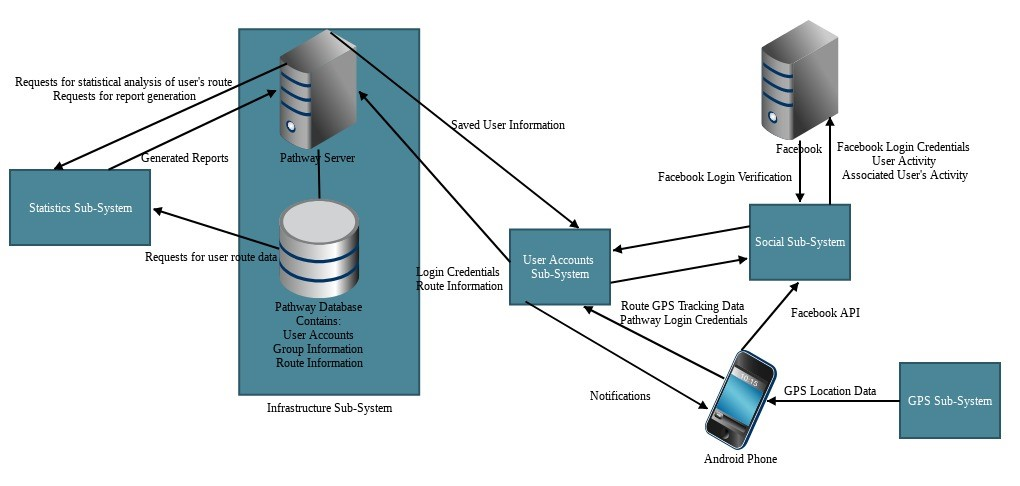
\includegraphics[width=\textwidth]{system_model.jpg}
    \caption{System Model}
    \label{fig:my_label}
\end{figure}

\pagebreak


\section{Application Structure And Flow}
\subsection{Pathway Structure}

Pathway will be comprised of five primary components, as shown in the System Model in Figure 1:
\begin{enumerate}
    \item Database Backend
    \item User Accounts
    \item Social Interaction
    \item Geolocation
    \item Statistics
\end{enumerate}
The above systems are detailed in full in their respective subsections in Section 3: Sub-Systems of this report, but will we will briefly outline the functionality of each here and discuss their high-level interaction with one another.

The Database backend subsystem will serve as the data foundation for the application by providing data storage and look-up crucial for the functionality of all other subsystems. Each subsystem will interact with the database through an API developed for the application to facilitate passing of data back and forth.

The User Account subsystem will provide each user with a persistent experience across the application while maintaining account security for each user, ensuring that user data is correct, retrievable, and secure.

The Geolocation module will provide the primary functionality of the application, which is the collection of geographic route data associated with a user account and used in the Statistics subystem. This subsystem relies heavily on device sensors to generate accurate data as well as several web services to supplement the collected data.

The Social system will make use of the Facebook API to provide social networking features to users of the app, and is the primary avenue of motivation provided by the app, through social interaction.

Finally, the Statistics subsystem will be how the application allows users to derive and track useful information from repeated workouts. Using collected route data, users will be able to analyze performance metrics.

\subsection{Pathway Flow}
The Database system will necessarily communicate with systems at some point in the execution cycle of the application. Further, the Social and User systems will be dependent on each other, while also retrieving information from Statistics as needed.
The Statistics module will rely on data collected by the Geolocation module and saved account data from the Users module to calculate metrics.

\begin{figure}[!htb]
    \centering
    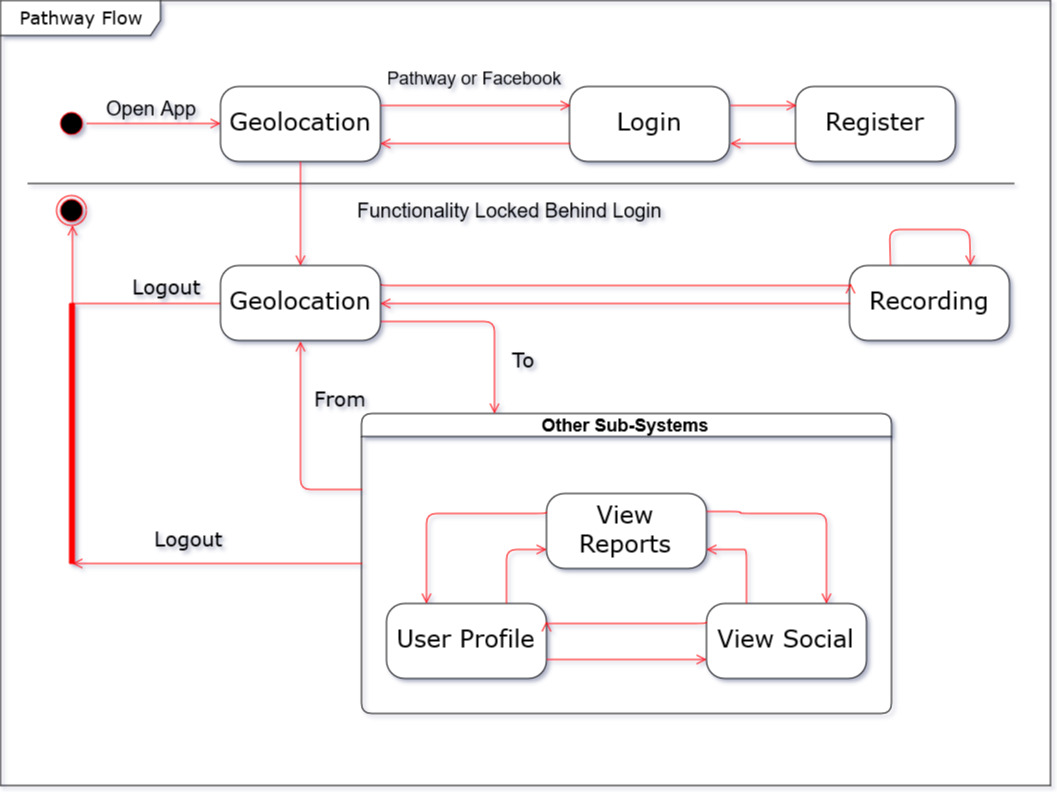
\includegraphics[width=\textwidth]{systemFlow.jpg}
    \caption{System Flow}
    \label{fig:my_label}
\end{figure}

\subsection{UI Description}
Pathway will rely on 
Figure 2. may also be used to describe a general flow of the user interface, which is as follows:
\begin{enumerate}
    \item Upon loading the application, the user is met with a login screen and prompted to login.
    \item If the user has an account, they may login directly.
    \subitem If unsuccessful, the user is returned to the login prompt.
    \subitem If successful, the user is taken to the main UI fragment, the geolocation fragment.
    \item New users will be prompted to register, using either Pathway or Facebook.
    \item The geolocation module depicts a map with the users location, routes in the immediate vicinity, and a start button.
    \item If the user presses start, the application begins recording user location and draws it to the map.
    \subitem User can record from the start of an existing route if tapped.
    \item From the map view, the user may use a drawer panel to navigate to their profile, a summary of their social page, or metrics for the user and/or current route.
    \item From any of these views, the user may navigate to all other views using the navigation drawer.
    \item From the navigation view, user may select logout to be taken back to the login screen.
\end{enumerate}

\section{User Requirements}
\subsection{Functional}
\begin{enumerate}
    %%
    %% New user requirements
    %%
    \item Request an account be created.
    \item Request that an account be logged into.
    \item request that an account be logged out.
    \item delete/remove an account, with appropriate privilege levels.
    \item update an account's information.
    \item create a route in the database.
    \item delete a route in the database.
    \item update a route in the database.
    \item query for statistical calculation on a user's data.
    \item The user will be able to link their Facebook account with the app to create an account
    \item The user will be able to fill out a form based application to create an account
    \item The system will allow the user to challenge other users within their area through the application interface
    \item Users will be able to compete for best time on routes in their area
    \item The system will be designed to accommodate future updates and additional functionality as needed.
    \item The system will be available for constant use, except during a small as of yet undetermined timeframe to allow for system maintenance and updates.
    \item The system will be stable, minimizing application crashes, freezes, or “hang-ups”.
    \item The system must be energy efficient with respect to the mobile device.
    \item The system must be efficient with respect with to cellular data consumption.
    \item If Facebook is down the account integration feature in the app will be expected to have downtime as well.
    \item The system will use collected geospatial data and user demographic information to present analysis of the user’s performance.
    \item The system will take user data and generate leaderboards for heavily used routes incertain areas, in order to allow users to compete for bragging rights on those routes.
    \item The system will generate a report after a run detailing the user’s performance with comparisons of previous runs.
    \item The system must generate reports that should be easily readable and detailed while avoiding being confusing to users.
    \item System will use device sensors to record GPS data in a Latitude/Longitude format.
    \item System will use device sensors to record user elevation.
    \item System will plot Geolocation data against a Google provided background map.
    \item System will record relative time stamps to use in calculation of speed and direction.
    \item System will display user activity duration, speed, distance, current elevation, and coordinates during data collection.
    \item System will display user routes clearly and in real-time as data is being collected.
    \item System will allow the user to save individual routes to a comma-delimited file for personal use.
    \item System will display traversed routes in the User's immediate vicinity.
    \item System will allow a user to tap on a route to retrieve and view information associated with that route.
    \item System will store a user’s routes in a particular format for use in Pathway.
    \item System will maintain a local device database to store a user's route data.
    \item System will be available as long as a persistent data connection is allowed.
    \item System will be made available in a limited capacity with reduced accuracy and no map service while no data connection exists.
    \item System will accurately and precisely locate the user’s position within an acceptable margin of error, allowing for a larger margin where service is weak or none exists.
    \item The System will allow the user to create an account that will be kept up to date by the system.
    \item The system for user accounts will keep track of a user's life time statistics and display them in an always up to date state, statistics include, life time steps, distance, best course, best time, etc.
    \item The user accounts system will save all user routes in the appearance of a fanned stack of cards.
    \item The system will allow the user to pull up these saved routes and see their best time or if that time has been beaten by anyone that they have shared it with.
    \item The system will also create graphs that display the user’s progression over time of running a route, that user can see.
    \item The system will be designed to accommodate future updates and additional functionality as needed.
    \item The system will be available for constant use, except during a small as of yet undetermined timeframe to allow for system maintenance and updates.
    \item The system will be stable, minimizing application crashes, freezes, or “hang-ups”.
    \item The system must be energy efficient with respect to the mobile device.
    \item The system must be efficient with respect with to cellular data consumption.
    \item The system must generate reports that should be easily readable and detailed while avoiding being confusing to users.




\end{enumerate}
\subsection{Quality}
\begin{enumerate}
    \item The system will be designed to accommodate future updates and additional functionality as needed.
    \item The system will be available for constant use, except during a small as of yet undetermined time-frame to allow for system maintenance and updates.
    \item The system will be stable, minimizing application crashes, freezes, or “hang-ups”.
\end{enumerate}
\subsection{Platform}
The client application will be written to support a minimal android version of 5. The back end will be built using Python3 and Flask, and will run inside of a Docker container. The database itself will be written in Python, MySQL, and SQLAlchemy and will also be housed inside of a Docker container. The container itself will be hosted on an Amazon Web Services (AWS) instance. The tracking and mapping of routes will be implemented through the use of the Google Maps API, and the statistical analysis of user data will be implemented with Python3 and Java, where necessary. The systems to provide statistical analysis will also be housed along with the back-end application.
Specific technologies should be listed here, including version numbers of languages.

\subsection{Process}
The project will be completed over the course of the Fall 2017 semester, with regular progress updates provided every few weeks. We are currently deciding upon a software engineering methodology to follow, such as agile methodologies. As we near the actual development phase we will settle upon a methodology to adhere to.

\section{Sub-Systems}

\subsection{Back-end Infrastructure - Cory Sabol}
\subsubsection{Introduction}
The Infrastructure subsystem of the Pathway application is responsible for providing a stable API by which the client application
can access, create, and update data stored in the database, which is also a part of the infrastructure subsystem. The API exposed also
provided a means for the client application to query for various statistics that are calculated server side. However these functions aren't
a part of the subsystem, they are their own subsystem which is merely housed on the server.

\subsubsection{User Requirements}
We will refer to any client application which may consume the API as a client from this point forward. The word "user" will refer to a person which may utilize the
Android application and services provided by Pathway. Below is a list of the user/functional requirements that the infrastructure subsystem will satisfy. These are all actions performed by a client, not a user.
\begin{enumerate}
    \item Request an account be created.
    \item Request that an account be logged into.
    \item request that an account be logged out.
    \item delete/remove an account, with appropriate privilege levels.
    \item update an account's information.
    \item create a route in the database.
    \item delete a route in the database.
    \item update a route in the database.
    \item query for statistical calculation on a user's data.
\end{enumerate}

\subsubsection{Platform Requirements}
To implement the subsystem described in this document, the platform required must support standard HTTPs connections, be stable, and provide a
way to establish RESTful architecture. That is why the following tools have been chosen.

\begin{itemize}
    \item Python version $\geq$ 3, to write server side logic.
    \item Flask, to provide a simple, scalable web server that utilizes python.
    \item MySQL, to provide the database to house all user and application data.
    \item SqlAlchemy, to provide an Object Relational Mapper (ORM) for accessing the database in a more efficient and secure manner.
    \item Docker, to isolate the application in a consistent environment which can easily be moved from development to deployment.
    \item Amazon Web Services (AWS), to provide the physical server architecture needed to host a centralized server application.
\end{itemize}

\subsubsection{Domain Analysis}

\paragraph{Introduction}
The following sections are devoted to examining the domain which the infrastructural subsystems of the Pathway application reside.

\paragraph{Extensions}
The infrastructure for the Pathway project isn't necessarily extensible in the same way that the other subsystems are.
However, it could be extended by making it more scalable. This would allow the system to be
more redundant and support a larger volume of users. In addition to scalability, the system by it's nature, will have to be extended
along with most extensions that could take place within the other subsystems.

\paragraph{General Domain Knowledge}
This susbsytem falls into the category of backend web development, which is a domain that the developer already has a sizable amount of professional exeperience in.
\begin{itemize}
    \item Because HTTP is transactional, a REST api incurrs some network overhead.
    \item Python is a language which facilitates rapid development. Making it great for a web service.
    \item The flask framework isn't particularly well suited to handling large volumes of requests. Meaning we would
    need to port to a web server which scales better should we have a user base increase.
\end{itemize}

\paragraph{Clients and Users}
The only clients that this subsystem can have are any applications which consume it's API. In the case of Pathway this will be all
of the other subsystems which make up the native Android application.

\paragraph{The Environment}
The computing environment for this subsystem will be an Ubuntu 14.04 instance which has been dockerized. This will be deployed to an AWS instance. The purpose of running the server side code in a docker container is that docker allows us to tailor the OS environment
to cater specifically to the application. Which provides a more isolated development and production environment for the code, minimizing variables which could contribute to bugs and other such undesirable behaviors.

\paragraph{Tasks and Procedures}
This subsystem does not replace an real world tasks or procedures. It is more like the glue which allows the application to
network with other instances of the application and to house and retrieve data.
\begin{itemize}
    \item Receive incoming HTTP requests.
    \item Process data sent to API endpoint via HTTP request.
    \item Respond to HTTP requests which were successfully received.
    \item Update the database.
    \item Provide user authentication.
\end{itemize}

\paragraph{Competing Software}
Because this subsystem, by nature of it's purpose, is customized to facilitate the possibility of the actions that the client Pathway
application provides, there is not necessarily any competing software.

\paragraph{Domain Similarities}
Other applications may require a backend which is similar to the backend for Pathway.
\begin{itemize}
    \item Other fitness applications such as Strava.
    \item Other social applications such as Facebook, or Twitter may have similar backend logic.
\end{itemize}

\subsubsection{System Analysis}
\paragraph{Introduction}
This document describes the planning and analysis of the infrastructural subsystem of the
Pathway project. Which encompasses the database, server logic and houses several other subsystems
by providing an interface for various client side systems to access.

\paragraph{Process Model}
Since this subsystem is not necessarily an entirely programmer created system, but rather a
composition of application environments and configurations as well as primarily declarative
logic to handle server routing, the high-level behaviour and structure of the system is best
described using a sequence diagram rather than UML class descriptions. \textbf{Figure 2} shows
a sequence diagram of the backend systems. It also describes environment encapsulation and which
system objects belong to which tools.

\begin{figure}
    \centering
    \begin{center}
        \makebox[\textwidth]{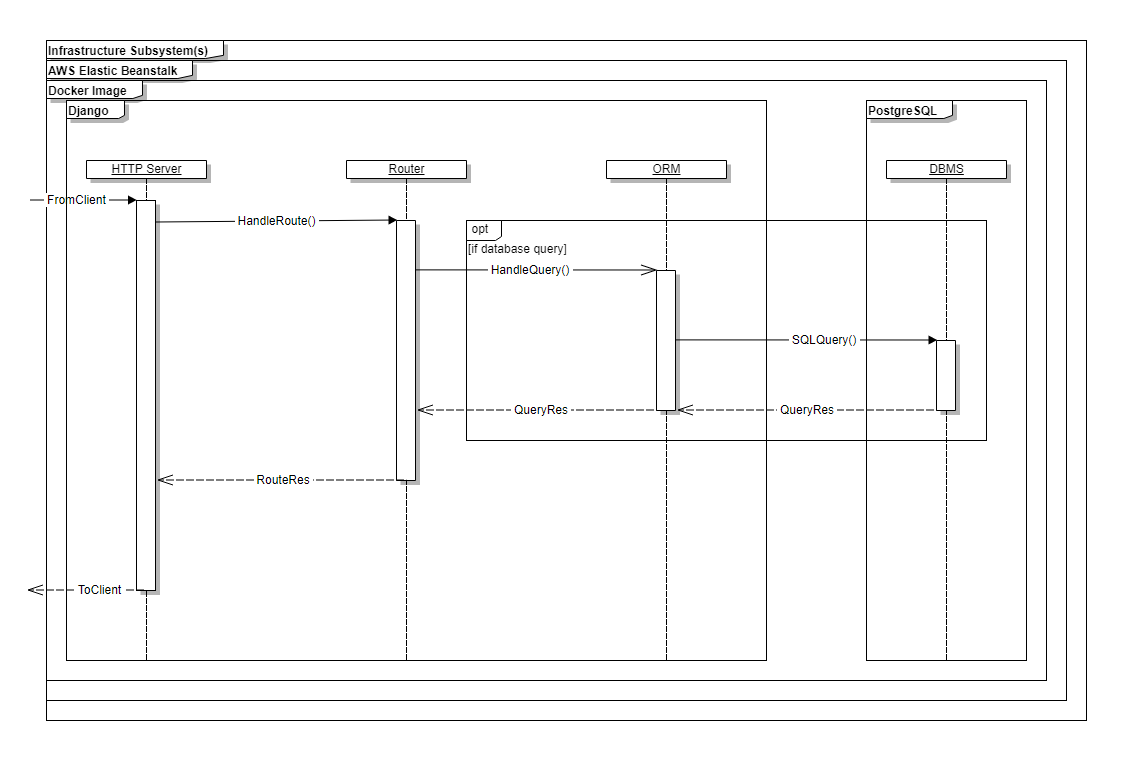
\includegraphics[width=\paperwidth]{PWInfSeq.PNG}}
    \end{center}
    \caption{Pathway Backend Sequence Diagram}
    \label{fig:my_label}
\end{figure}

\paragraph{Detailed Model}
\paragraph{System Analysis}
Detailing the model of the infrastructure really comes down to describing how the
various components communicate with one another, and with other systems.
The server itself communicates with the database via and ORM system, which is built into
Django. The server can be communicated with the following example API;

\begin{enumerate}
  \item API Example (not a full definition of the API)
    \begin{enumerate}
      \item /auth - handle user authentication and deauthentication
        \begin{enumerate}
          \item /login - POST the user login data
          \item /logout - POST request to logout current user, destroys session.
          \item /create - POST create an account from posted data
          \item /deactivate - POST deactivate user account (requires authentication)
        \end{enumerate}
      \item /users - GET all users
        \begin{enumerate}
          \item /[userName] - GET user summary belonging to userName
          \item /[userName]/[routes,stats,profile] - GET routes or stats or profile of userName
        \end{enumerate}
      \item /routes - GET all routes (paginated)
        \begin{enumerate}
          \item /[routeId] - GET specific route
        \end{enumerate}
    \end{enumerate}
\end{enumerate}

Clients may directly craft and send http requests to the API endpoints, or java based
applications may leverage the java library which is a wrapper to the server's API. This is
the recommended approach, as it abstracts the work of making http requests and handling the
responses into a native library which exposes an interface of functions and it's own types.

\paragraph{System Analysis}
Since this subsystem relies heavily on both a webserver framework and a DBMS which means that
we do not face the same challenges in determining efficient solutions that we do when we define
and develop algorithms. The implementation of the webserver and the DBMS are hidden away from us,
therefore we must consider which tools at our disposal are the best for our purposes. Rather
than analyze specifically for algorithm efficiency (although we will do this should the need
arise), we will focus on issues such as scalability, redundancy in the database, environment set up,
resource size (how much data are we sending to the client and vice versa), concurrent connections, and
many other challenges to explore.

\paragraph{Use Cases}
With respect to this subsystem a client refers to any application which interfaces with this subsystem.
\begin{enumerate}
\item A client wishes to authenticate a user.
    \begin{enumerate}
        \item Client makes call to 'auth/' API endpoint, passing username and password over HTTPs.
        \item Subsystem authenticates username and password using the User Account subsystem.
        \item Subsystem sets the client session to authenticated or non-authenticated.
    \end{enumerate}
\item A client deauthenticate a user.
    \begin{enumerate}
        \item Client requests to be deauthenticated.
        \item System destroys client session.
    \end{enumerate}
\item A client wishes to store a new route in the database.
    \begin{enumerate}
        \item Client makes a POST request to '/route/add/', with the route data in the body.
        \item Subsystem stores route in database via ORM.
    \end{enumerate}
\item A client removes a route from the database.
    \begin{enumerate}
        \item Client makes GET request to '/route/del/[id]' with the id of the route to delete.
        \item Subsystem drops route from the database.
    \end{enumerate}
\item A client updates a user profile.
    \begin{enumerate}
        \item Client make POST request to '/user/profile/update' with user profile data blob in request body.
        \item Subsystem makes appropriate update to user entry in database.
    \end{enumerate}
\item A client requests a report on user data.
    \begin{enumerate}
        \item Client makes GET request to '/report/[type]/[date]' with report type and data in the url.
        \item Subsystem passes type and date to the statistic subsystem to generate the report.
        \item Subsystem returns report data as JSON string.
    \end{enumerate}
\end{enumerate}

\paragraph{Scalability}
Scalability is one of the largest challenges that is faced when developing a web based application
as well as development time. For this system, it needs to provide access to a database as well as
expose a RESTful API and an admin page. There are two choices that make sense here with respect to
providing these features and reducing development time; Django and Flask. These two tools imply that
we have decided to utilize Python3 on the server side, for it's ease of use. Django and Flask are
both python based web frameworks, which provide essential HTTP functionality. However, Flask is
much smaller than Django and provides less out of the box. Meaning that more developer effort is
required to implement the features that we desire. Django on the other hand, is very much a
"batteries included" framework. It provides several key things out right; an ORM, REST plugin,
admin tools/pages, and deep database integration, and robust security options. This makes it the
choice of web framework for the Pathway project (other security implications?). Django is also
built with scalability in mind.

\paragraph{Hosting}
When developing an application which requires a back end server, it's also important to realize that
hardware is required in order to actually host the application. The choices for this come down to
Amazon Elastic Beanstalk or Heroku. Both of these services provide similar things. Hosting of
web applications, and their databases, as well as management/admin tools. However, Elastic Beanstalk
is somewhat cheaper as a student, and provides better load balancing tools, which is important
should the service ever need to scale according it's userbase. There is a big difference between
1000 concurrent users, and 10,000. Amazon web services has a great track record of being an
industry standard when it comes to deploying hosting applications which may need to scale and
handle large numbers of connections. The drawback to Beanstalk versus Heroku is that Heroku is
vastly easier to use and interface with from a developer standpoint.

\paragraph{Database}
Choice of database is a very important choice as well. For this decision however we have opted to
go with the choice which aligns best with ease of setup and lowering developer time. PostgreSQL
has very tight integration with Django, and there are extensive community resources with regard to
it. At this stage of the project, the database schema is relatively simple, and it will certainly
be expanded upon as we continue to develop. \textbf{Figure 2} shows the database schema.

\begin{figure}
    \centering
    \begin{center}
        \makebox[\textwidth]{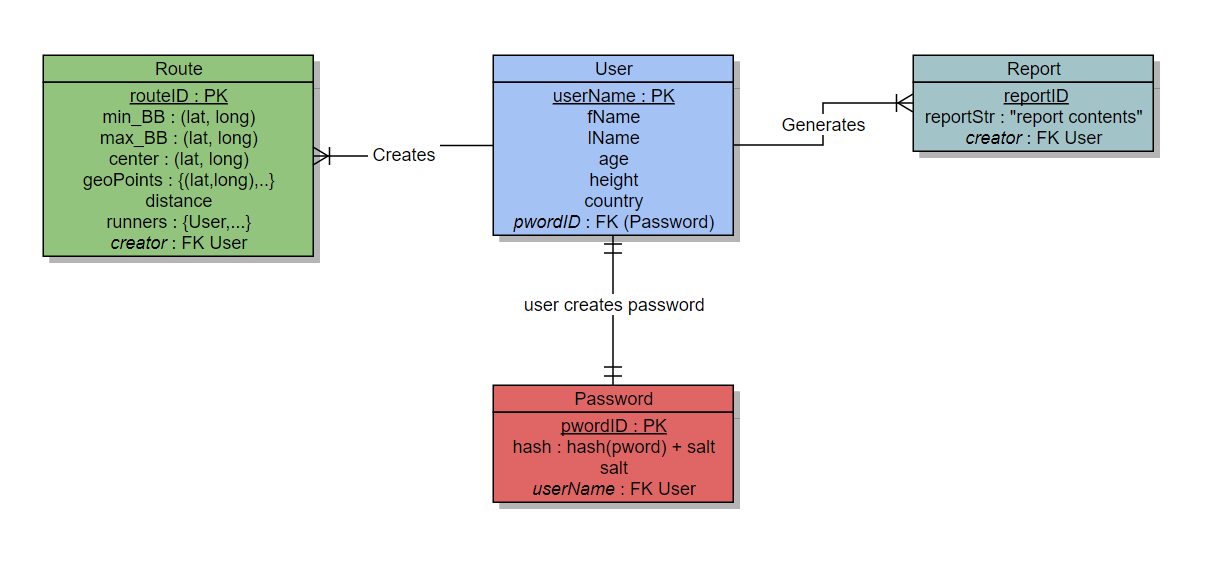
\includegraphics[width=\paperwidth]{ER.png}}
    \end{center}
    \caption{Pathway Database ER Diagram}
    \label{fig:my_label}
\end{figure}

\paragraph{Classes}
There isn't much to discuss here, the only classes which will be developed for the infrastructure
will be classes for the ORM (object relational mapper). These classes will be essentially be 1:1
with the tables described in \textbf{Figure 2}. These classes will make use of the Django models
library, and will be used in the actual construction and initialization of the database.

\paragraph{Deployment}
Lastly deployment from development to production is a complex topic worth study of it's own.
For this challenge we could either create an isolated development environment with a tool like
Docker, which will allow us to have a localized development environment which can mimic the
production environment as well as being fully scriptable, or we could have each developer install
python3, Django, PostgreSQL and any other tools to their machine and fight with inconsistencies
across each machine. The choice here is pretty obvious. We have opted to utilize Docker to
provide an isoloated development and testing environment which contains exactly the tools necessary
for the server applicaiton and database to run. This would only require that each developer
use the Docker build script to build the image on their machine, and then develop and test against
it. Amazon Elastic Beanstalk also has support for deploying dockerized applications.

\paragraph{Tool Selection}
\begin{itemize}
    \item Docker
    \item Django
    \item Python3
    \item PostgreSQL
    \item Amazon Elastic Beanstalk
\end{itemize}

\subsubsection{Selected Source Code}
\paragraph{Serializers}
\begin{lstlisting}[language=Python]
from django.contrib.auth.models import User, Group
from rest_framework import serializers

class UserSerializer(serializers.HyperlinkedModelSerializer):
  class Meta:
    model = User
    fields = ('url', 'username', 'email', 'groups')

class GroupSerializer(serializers.HyperlinkedModelSerializer):
  class Meta:
    model = Group
    fields = ('url', 'name')

class RoutrSerializer(serializers.HyperlinkedModelSerializer):
  class Meta:
    model = Route
    fields = ('routeID', 'dateCreated', 'creator', 'geoData')
\end{lstlisting}

\subsubsection{Views}
\begin{lstlisting}[language=Python]
from django.shortcuts import render
from django.contrib.auth.models import User, Group
from rest_framework import viewsets
from pathwayserv.api.serializers import UserSerializer, GroupSerializer

# Create your views here.

class UserViewSet(viewsets.ModelViewSet):
  '''
  API Endpoint that allows users to be viewed or edited.
  '''
  queryset = User.objects.all().order_by('-date_joined')
  serializer_class = UserSerializer

class GroupViewSet(viewsets.ModelViewSet):
  '''
  API Endpoint that allows groups to viewd or edited.
  '''
  queryset = Group.objects.all()
  serializer_class = GroupSerializer

class RouteViewSet(viewsets.ModelViewSet):
  '''
  API Endpoing to handle creation and viewing of routes
  This is currently undefined.
  '''
\end{lstlisting}

\paragraph{Docker File}
\begin{lstlisting}[language=Bash]
FROM python:3

MAINTAINER Cory Sabol
ENV PYTHONUNBUFFERED 1
RUN mkdir /code
WORKDIR /code
ADD requirements.txt .
RUN pip install -r requirements.txt
ADD . /code/
\end{lstlisting}

\paragraph{Docker-compose File}
\begin{lstlisting}
version '2'

services:
  db:
    image: postgres
  web:
    build .
    command: python3 manage.py runserver 0.0.0.0:8000
    volumes:
      - .:/code
    ports:
      - "8000:8000"
    depends_on:
      -db
\end{lstlisting}

\paragraph{Test Cases}
We can see that the selected code snippets satisfy several of the test cases, which we define
as use cases that have been backed by working code. Currently the code for the infrastructure
subsystem satisfies several test cases, some more concrete than others.
\begin{itemize}
\item The system accepts HTTP requests and is capable of responding via HTTP.
\item The system is able to handle the creation of a user.
\item Viewing of users in serialized json format is also handled.
\item Groups may also be created.
\item Groups may also be viewed.
\item The system has communication with the database.
\item The system satisfies the need for administration with admin users and an admin portal.
\item The system supplies a contained development environment which mimics production.
      i.e the system is deployable and meets the criteria for a sane development pipeline.
\end{itemize}

While this is not a full overview of the system, it is fully ready to supply a robust
API and backing for the Pathway mobile application. The API only needs to be defined
from it's current point. Team member which need to develop applications against the API
or develop systems which run on the server need only run a local instance by utilizing
Docker which is configure to run a version of the server application that is local to the
developers machine and a database which is a clean slate for every developer. Once
a version of the application is complete, the source and the docker configs can be deployed
to an AWS instance, where the docker image will be built and the application server started.

\paragraph{Data Conversion Plan}
Since this subsystem is the one which houses the data and provides access of the data to other systems,
a conversion to a new implementation system or even server hardware would not affect the other subsystems.
Only an API revision would trigger a possible need for a change in the way that the other systems handle the
data belonging to the Pathway application.

This section is best explained with an example. If the need arose to build the server side
API application in a new language, it would be trivial due to the decoupled nature of all the
parts that comprise the entire subsystem. This is thanks to Docker, which allows the subsystem
to be built in interchangeable layers. Each layer effectively has it's own isolated OS in the form of
a docker image in which the relevant software runs. Each layer (container) communicates via a
network constructed solely for the containers which make up the application as a whole. Consider
an entire rewrite of the API layer from Python to Haskell (something which is plausible in the future).
This event would in no way affect the existing data in the database container, as the database container
is completely isolated from the API layer. The only changes that would cascade through all layers would
be changes to the database schema itself. This is because every other part of this subsystem depends upon it.


%=====================================================================================

\subsection{Social - Chris Carney}
\subsubsection{Introduction}
The Social subsystem will utilize some simplistic features that enable the user to interact with other users using the app within their local area. We will be implementing certain aspects from a Facebook API that will allow the user to integrate their Facebook profile when they first create an account that will let them expand their use of the app to include others. The user will also have a form based alternative to make a profile which would give the user an opportunity to create a profile straight from the app but would limit its inclusivity of other users and just be used to keep records of their routes that they recorded without any social aspect in place.
The app will give the users an option to choose a route in their specified location which will then list the top times that the route was traveled, then the user will be able to choose a top time that is displayed in the list and will be able to implement the “Challenge” function, which is similar to a “poke” on Facebook. After the user picks the time they want to “challenge” on a certain route, and they complete it, the person that the user chose to challenge would be notified if their time was beaten depending on if the user completed that route in a faster time.
We will also include an achievement system feature that will give incentives the user based on certain accomplishments within the app.

\subsubsection{User Requirements}
\begin{itemize}
    \item The user will be able to link their Facebook account with the app to create an account
    \item The user will be able to fill out a form based application to create an account
    \item The system will allow the user to challenge other users within their area through the application interface
    \item Users will be able to compete for best time on routes in their area
    \item The system will be designed to accommodate future updates and additional functionality as needed.
    \item The system will be available for constant use, except during a small as of yet undetermined timeframe to allow for system maintenance and updates.
    \item The system will be stable, minimizing application crashes, freezes, or “hang-ups”.
    \item The system must be energy efficient with respect to the mobile device.
    \item The system must be efficient with respect with to cellular data consumption.
    \item If Facebook is down the account integration feature in the app will be expected to have downtime as well

\end{itemize}

\subsubsection{Platform}
\begin{itemize}
    \item The system will be developed using Android v5 (Lollipop).
    \item The system will be developed in Android Studio.
    \item The system will employ the Facebook API.
\end{itemize}

\subsubsection{Domain Analysis}
\paragraph{Extensions}
\begin{itemize}
    \item Increased social networking functionality.
    \item Broaden integration for other social network sites such as Twitter and Instagram.
\end{itemize}

\paragraph{General Domain Knowledge}
While many individuals like to share their workout information on social media sites, there does not currently exist an integrated fitness oriented social networking option.

\paragraph{Clients and Users}
\begin{itemize}
    \item Targets users capable of operating a compatible device that this application could be installed on.
    \item Facebook Users.
\end{itemize}

\paragraph{Computing Environment}
Primary functionality will be coded in Android 5.0 (Lollipop) and as such will be unsupported on older versions of Android. Specific system requirements are not yet determined. No additional client requirements will be necessary for database access, other than an active connection to internet.

\paragraph{Tasks and Procedures}
\begin{itemize}
    \item Linking Facebook account to the app: The app will ask if the user has a Facebook account they would like to link upon account creation.
        \subitem This will prompt Facebook to authorize permission for the app to access its functionality such as sharing posts straight from the app.

    \item User “Challenges” a record time on the leaderboard for a route: User chooses a route within their area, which then lists the top times that the route was completed.
        \subitem User has option of picking what time they would like to challenge.
        \subitem Upon completion of the route, if the user who challenged the time completes the course in a shorter time, then the user that was challenged would receive a notification that their time was beaten.
\end{itemize}

\paragraph{Competing Software}
The following applications/software may fulfill similar roles or offer similar functionality:
\begin{itemize}
    \item MyTracks - Offers only basic data collection (Lat/Long position, elevation) dependent on device sensors, and no analysis options.
    \item FitBit App - Offers data collection and basic analysis of user performance.
    \item iOS Health - Offers basic data collection and limited analysis of performance.
    \item LG Health - Offers route tracking and calorie journal. Still lacks any social networking component.
\end{itemize}

\paragraph{Similar Domains}
Many applications are similar to Pathway in the sense that they make use of geospatial data location and/or social networking user accounts. While no other application we found combines all aspects of our project in the same way we do, it will be worthwhile to look at other applications, such as Waze, Facebook, and other apps to gather some understanding of how to efficiently implement these systems.

\subsubsection{System Analysis}
\paragraph{Introduction}
Since the User Accounts subsystem will be focusing on implementing the choice to create a profile through the app, the Facebook API will be the majority of what we will be using in this subsystem to help authorize a user’s profile and also gain access to the users profile information given the option to control what permissions the user will be able to access from the app whether it be from their personal info to their friends lists.

In order to do this, we will first need to utilize a program called OpenSSL. OpenSSL is a software library for applications that secure communications over computer networks from being accessed by unauthorized users. It contains an open-source implementation of SSL and TLS protocols. It's core library implements cryptographic functions and provides various utility functions. OpenSSL also utilizes wrappers which allows its library to be used across many different computer languages so that there are no compatibility issues. With OpenSSL, we will be able to obtain a key hash. A key hash is a 28-character string that Facebook uses to authenticate any type of exchanges of information in between Facebook and the Pathway app. If a key hash is not obtained, there will be no possibility of Facebook integration within the app.

After establishing the connection to the users Facebook account, we will be implementing the CallbackManager class provided by the Facebook API which determines how methods are called and what values are returned from those methods which will interact with other classes within the Social subsystem while also interacting with each of the other subsystems. During this process, we have the option to list what permissions the app will have access to such as the user's basic profile information, email, or list of friends. This is how we plan to get access to the user's list of friends that also have the app installed which is already determined through the Facebook API.

\begin{figure}[H]
      \centering
      \begin{center}
            \makebox[\textwidth]{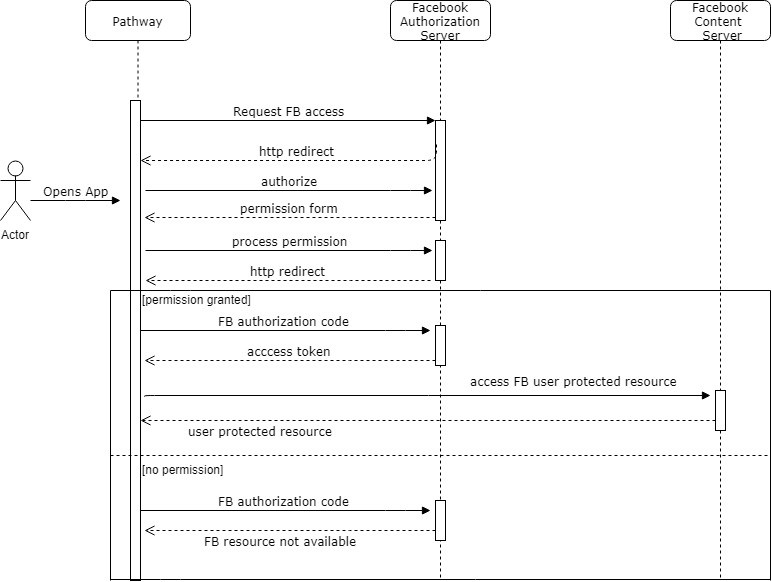
\includegraphics[width=0.8\paperwidth]{carney01.jpg}}
        \end{center}
      \caption{Pathway social sequence diagram}
      \label{fig:my_label}
  \end{figure}

\begin{figure}[H]
      \centering
      \begin{center}
            \makebox[\textwidth]{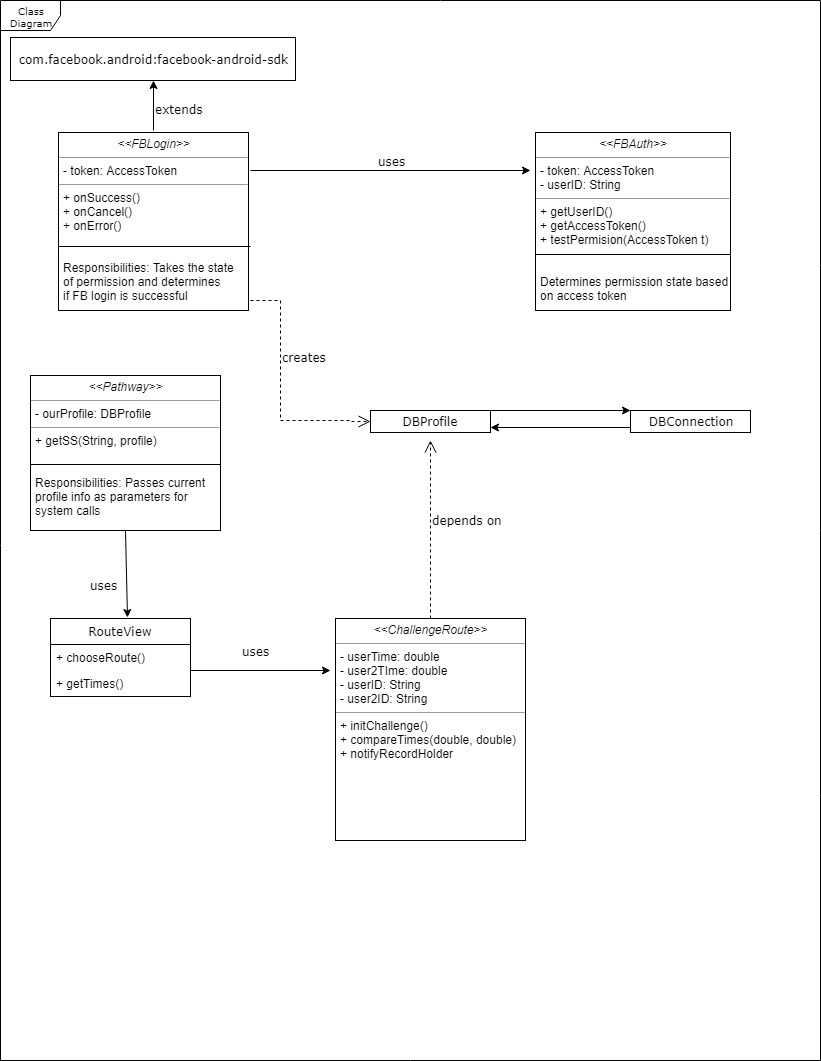
\includegraphics[width=0.8\paperwidth]{carney02.jpg}}
    \end{center}
    \caption{Pathway social UML diagram}
    \label{fig:my_label}
\end{figure}

\begin{figure}[H]
    \centering
    \begin{center}
        \makebox[\textwidth]{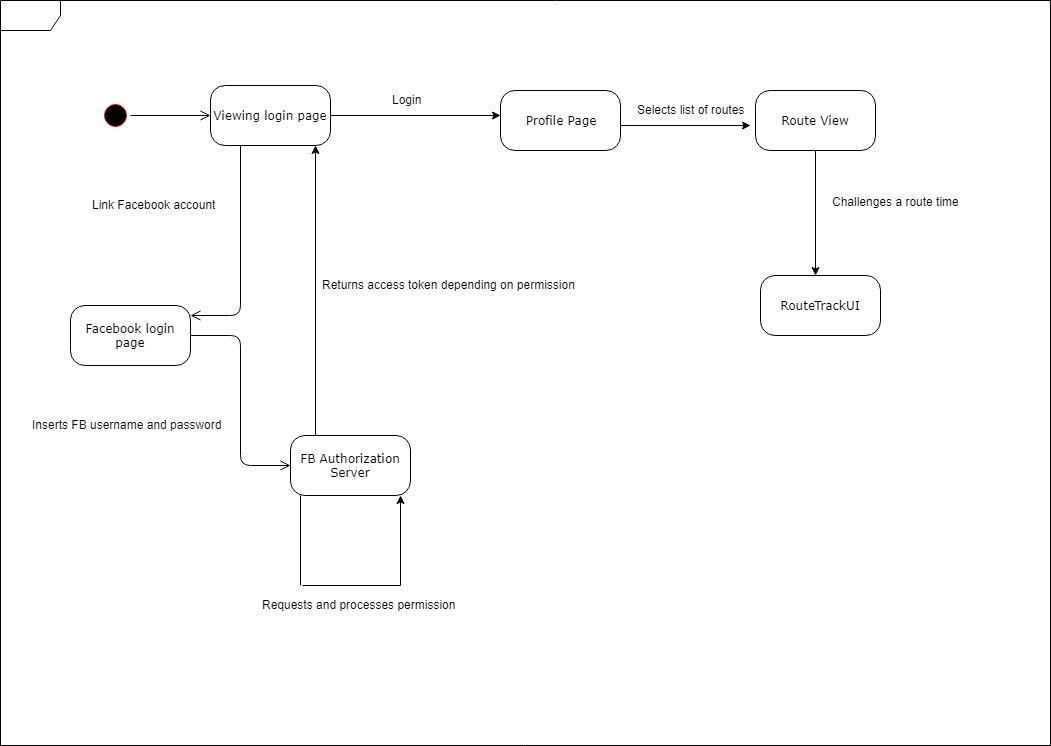
\includegraphics[width=0.8\paperwidth]{carney03.jpg}}
    \end{center}
    \caption{Pathway social activity diagram}
    \label{fig:my_label}
\end{figure}

\begin{figure}[H]
    \centering
    \begin{center}
        \makebox[\textwidth]{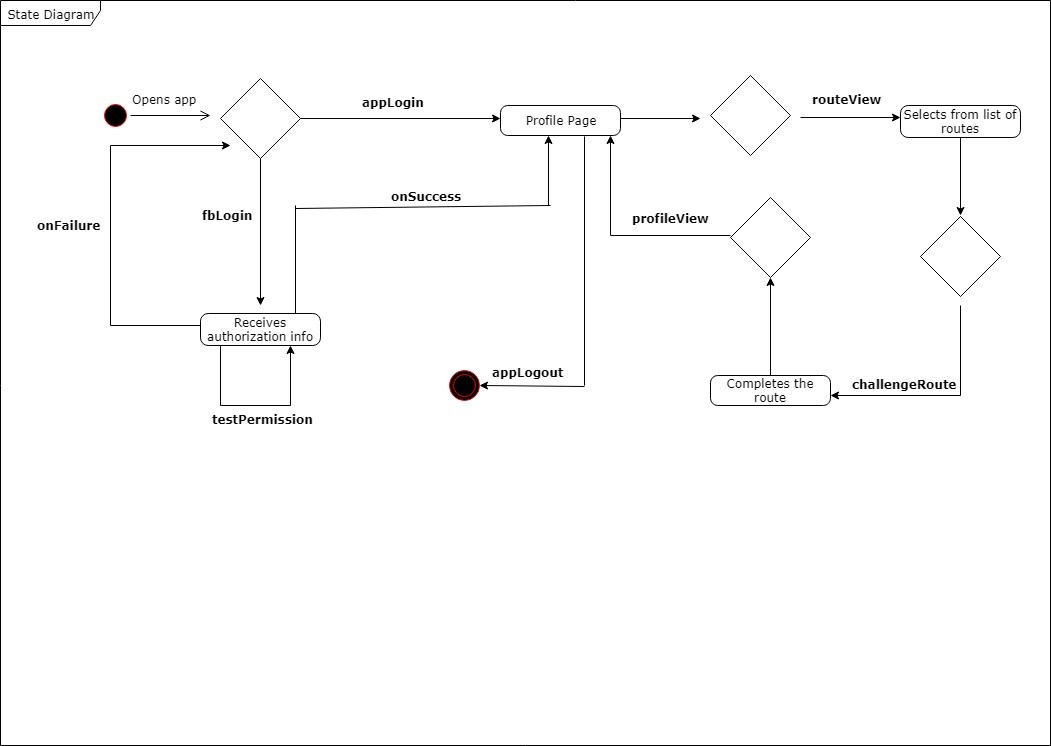
\includegraphics[width=0.8\paperwidth]{carney04.jpg}}
    \end{center}
    \caption{Pathway social state diagram}
    \label{fig:my_label}
\end{figure}

\begin{figure}[H]
    \centering
    \begin{center}
        \makebox[\textwidth]{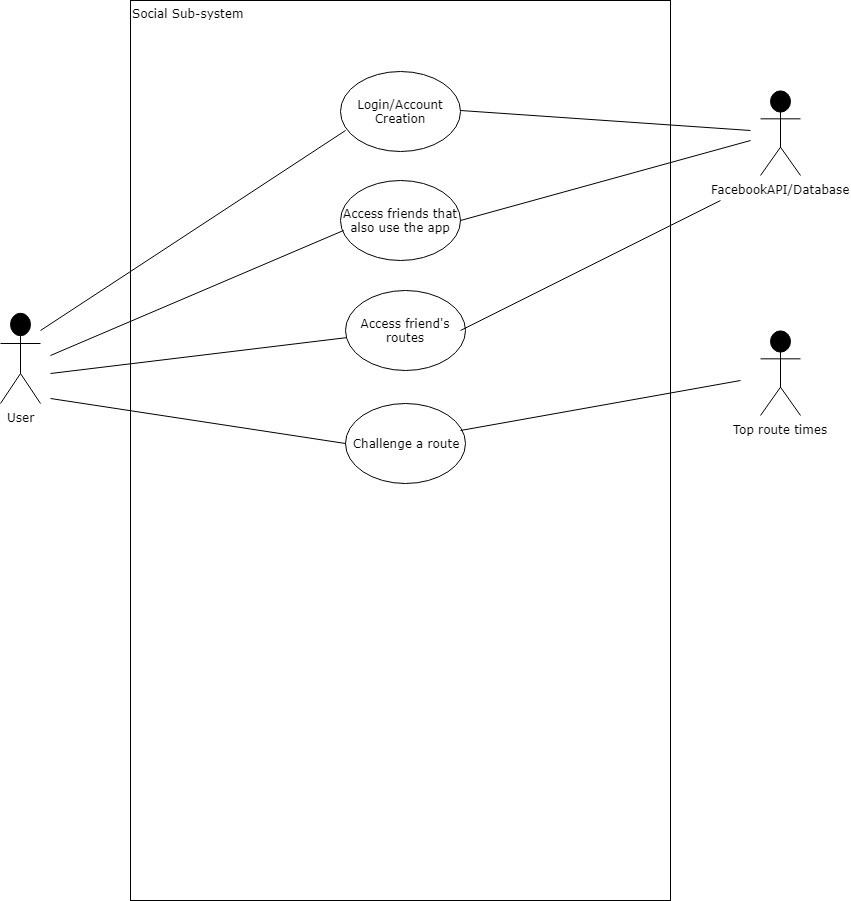
\includegraphics[width=0.8\paperwidth]{carney05.jpg}}
    \end{center}
    \caption{Pathway social use case diagram}
    \label{fig:my_label}
\end{figure}

\paragraph{Use Cases}
\begin{enumerate}
\item The user creates an account:
    \begin{enumerate}
    \item The user wishes to use Pathway and creates an account either through linking their facebook account or by making an account through our system.
    \end{enumerate}
\item The user logs in:
    \begin{enumerate}
    \item The user has an account and wishes to login, they either enter their credentials or select to login using their facebook.
    \end{enumerate}
\item The user wishes to challenge a “top time” on a route:
    \begin{enumerate}
    \item The user wants challenge a user that holds a record time for a route. After selecting a route from a list, the users can display the top times for that route and will have the option to “challenge” it
    \end{enumerate}
\item The user wishes to see friends from Facebook that also have the app:
    \begin{enumerate}
    \item The user hits the friends tab, and it loads all of their friends that also have the app installed on their device
    \end{enumerate}
\end{enumerate}
\pagebreak

+\subsubsection{Test Cases}
\begin{itemize}
  \item TC-01: Linking Facebook profile to app
  \subitem Requirements Fulfilled:
  \subsubitem The user will be able to link their Facebook account with the app to create
  an account.
  \subsubitem The app will be able to access the user's Facebook data in order to utilize other social functionalities
  \subitem Test Steps:
  \subsubitem 1. App is started.
  \subsubitem 2. Press "Connect with Facebook" button when prompted to login.
  \subsubitem 3. Webview of Facebook login page appears where the user will be prompted to enter their account email and password.
  \subsubitem 4. User will be directed back to app depending on whether the login was successful or not.
  \subitem Expected Result: User is logged in/registered and is added to the database with accessibility to core data such as name, email, and friend's list from Facebook account (other data can be accessed optionally).
  \subitem Actual Result: User is connected to their Facebook account but there is no UI set up for the main page of the app which is where the user will be directed once their Facebook login is successful.
\end{itemize}
\pagebreak

\subsubsection{Social Subsystem Code}
\paragraph{Facebook Login Code}
\begin{lstlisting}

import android.content.Intent;
import android.support.v7.app.AppCompatActivity;
import android.os.Bundle;
import com.facebook.AccessToken;
import com.facebook.AccessTokenTracker;
import com.facebook.CallbackManager;
import com.facebook.FacebookCallback;
import com.facebook.FacebookException;
import com.facebook.login.LoginResult;
import com.facebook.login.widget.LoginButton;

public class MainActivity extends AppCompatActivity {

LoginButton loginButton;
CallbackManager callbackManager;

protected void onCreate(Bundle savedInstanceState) {
super.onCreate(savedInstanceState);
setContentView(R.layout.activity_main);

//bind UI component to LoginButton variable
loginButton = (LoginButton)findViewById(R.id.login_button);
callbackManager = CallbackManager.Factory.create();

//sets permissions so that data from user's profile can be accessed
loginButton.setReadPermissions("email", "public_profile", "user_friends");

loginButton.registerCallback(callbackManager, new FacebookCallback<LoginResult>() {

//When login is successful
@Override
public void onSuccess(LoginResult loginResult) {
//code goes here
}

//When user cancels login
@Override
public void onCancel() {
//code goes here
}

//When an error occurs during login
@Override
public void onError(FacebookException error) {
//code goes here
}

});

}

@Override
protected void onActivityResult(int requestCode, int resultCode, Intent data) {
super.onActivityResult(requestCode, resultCode, data);

//callback manager gets response code to determine what next activity is
callbackManager.onActivityResult(requestCode, resultCode, data);
}

}

\end{lstlisting}

\paragraph{Achievement Implementation}
We have implemented simple achievements using UI components from Android Studio that the user can unlock by completing various actions within the app.  Our initial approach was to implement an achievement system using the Facebook API but certain restrictions hindered us from doing so. We will be creating a database table to hold boolean variables that correspond to the different achievements and are originally set to false. The Social Subsystem will be pulling information from the Statistics Subsystem to keep up with the user's progress toward each achievement. Once the information pulled from the user's statistics satisfies the requirement for an achievement, it will become unlocked. Below is the pseudocode for how each achievement will check for the boolean variable and change the status of the achievement.

\begin{lstlisting}
//code will make an HTTP GET request to the server to retrieve boolean variable
//then an if statement will check and see if requirements are satisfied for the achievement


if boolean variable is true{
	set achievement to "unlocked"
}

\end{lstlisting}

\newpage
%=======================================================================================

\subsection{Statistics/Metrics - Eric West}
\subsubsection{Introduction}
The statistics sub-system will perform analysis of user data generated by the Geolocation sub-system and data stored within the Infrastructure sub-system's database. This sub-system will take data generated from the use of the route tracking of the application and analyze it. It will then access the database by methods defined by the Infrastructure sub-system to retrieve any stored results that are related to this analysis compare and compare them to determine the user's performance. Once this is done the data will be organized into a formatted report and delivered to the User Accounts sub-system for reporting the details to the user. It will also allow the user to compare themselves to other users who have similar profile features. This sub-system will also generate any graphs of user data that are required by the user or by other sub-system.

\subsubsection{User Requirement}
\begin{itemize}
    \item The system will use collected geospatial data and user demographic information to present analysis of the user’s performance.
    \item The system will take user data and generate leaderboards for heavily used routes incertain areas, in order to allow users to compete for bragging rights on those routes.
    \item The system will generate a report after a run detailing the user’s performance with comparisons of previous runs.
    \item The system must generate reports that should be easily readable and detailed while avoiding being confusing to users.
\end{itemize}

\subsubsection{Platform}
\begin{itemize}
    \item The system will be developed using Python 3.
    \item The system will be a subservice housed along with the server application.
\end{itemize}

\subsubsection{Domain Analysis}
\paragraph{Competing Software}
The following applications/software may fulfill similar roles or offer similar functionality:
\begin{itemize}
    \item MyTracks - Offers only basic data collection (Lat/Long position, elevation) dependent on device sensors, and no analysis options.
    \item FitBit App - Offers data collection and basic analysis of user performance.
    \item iOS Health - Offers basic data collection and limited analysis of performance.
    \item LG Health - Offers route tracking and calorie journal. Still lacks any social networking component.
\end{itemize}

\paragraph{Extensions}
For later versions of this service we may try to increase the variety of analysis. We may also offer a web service allowing a more complete analysis of the user’s performance and physical activities.

\paragraph{General Domain Knowledge}
Few people have the knowledge or desire to manually formulate statistcs about their fitness progress.

\paragraph{Tasks and Procedures}
\begin{itemize}
    \item The user finishes a route.
    \item The user’s device uploads the route details up to the database on the server
    \item The server calls the statistic subsystem analysis function
    \item The function will be passed a way to access the data uploaded by the user
    \item The function will perform the analysis
    \item Determine average speed, distance, steps, etc.
    \item Analyze the routes gps points to determine the data points needed to plot a graph of distance over time
    \item Any extra data analysis involving previous route data
    \item Prepare information to be sent back to user
    \item Server sends the analysis data back to the user’s device
    \item Device will process the analysis data to generate a report for the user
    \item The report will display the average speed, steps, etc. for the route
    \item The device’s system will take the data points and plot a graph of distance over time.
\end{itemize}

\paragraph{Clients and Users}
This sub-system will be used by any device with the Pathway application and a user account.

\paragraph{Similar Domains}
There are many programs and applications that offer similar functionality to this sub-system. The nature of the application means that such sub-systems are required to fulfill the purpose of fitness tracking and personal improvement. It will be important to examine these other domains to learn how to improve and leverage more out of the sub-system.

\subsubsection{System Analysis}
\paragraph{Introduction}
For the statistics/metrics subsystem, the plan to utilize a python module specifically built to perform the necessary statistical operations, such as numpy.
This will be the most appropriate way to run the analysis as such modules are both efficient, fast, and well tested. This reduces the need to develop mathematical and statistical algorithms. This system will also use the json module to parse any JSON formatted data that is necessary to perform the calculations required of the system. The Python library Geopy will be used to determine distances for GPS points. On the client side, we will utilize a widely used library called Android Plot to render plots.
However the need to develop an efficient approach for handling the reports is necessary. For this reason we plan to implement the Factory method design pattern. This will allow the server to
simply pass a small amount of data to an object called a factory which contains methods that generate objects. This factory then gathers the necessary data from the database and performs the
various statistical calculations, such as determining averages and standard deviations, and passes this report to the server.

\paragraph{Use Cases}
Generate Report
\begin{enumerate}
\item User Requests report
    \begin{enumerate}
    \item App determines type of report to generate
    \end{enumerate}
\item Request is sent to server
\item Server processes request
    \begin{enumerate}
    \item The userID, routeID, and type of report are collected
    \item These values are passed to a ReportRequest object
    \end{enumerate}
\item ReportRequest is sent to ReportFactory
\item ReportFactory produces report with appropriate fields and plot values
    \begin{enumerate}
    \item ReportFactory determines behavior based on ReportRequest
    \item Requisite data is gathered by ReportFactory
    \item All necessary calculations are performed
    \item ReportFactory passes these values in a corresponding report-type object
    \end{enumerate}
\item Server sends report back to user
    \begin{enumerate}
    \item Server will audit report to ensure the report contains valid data.
    \item Sends the report
    \end{enumerate}
\item Pathway app processes the report
    \begin{enumerate}
    \item Report data is processed and passed into a structure to store and organize.
    \end{enumerate}
\item Processed report is displayed to the user.
    \begin{enumerate}
    \item Android activity will pull data from storage structure and fill in appropriate GUI components.
    \end{enumerate}
\end{enumerate}

\begin{figure}[H]
    \centering
    \begin{center}
        \makebox[\textwidth]{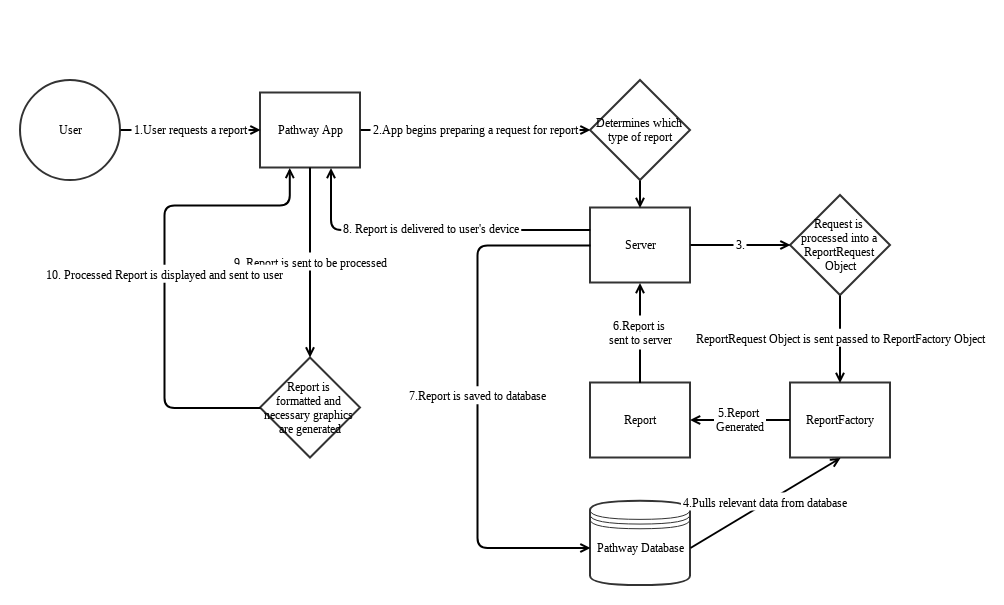
\includegraphics[width=\paperwidth]{westDF.png}}
    \end{center}
    \caption{Statistics system dataflow}
    \label{fig:my_label}
\end{figure}

\begin{figure}[H]
    \centering
    \begin{center}
        \makebox[\textwidth]{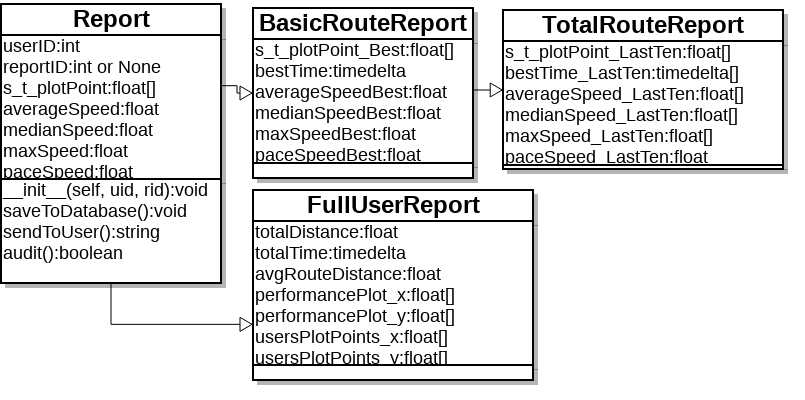
\includegraphics[width=\paperwidth]{westUML1.png}}
    \end{center}
    \caption{Statistics system UML:Report Classes}
    \label{fig:my_label}
\end{figure}
\begin{figure}[H]
    \centering
    \begin{center}
        \makebox[\textwidth]{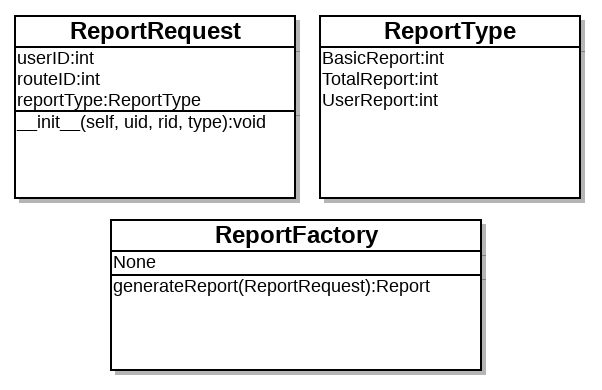
\includegraphics[width=\paperwidth]{westUML2.png}}
    \end{center}
    \caption{Statistics system UML: Utility Classes}
    \label{fig:my_label}
\end{figure}
\pagebreak


\begin{figure}[H]
    \centering
    \begin{center}
        \makebox[\textwidth]{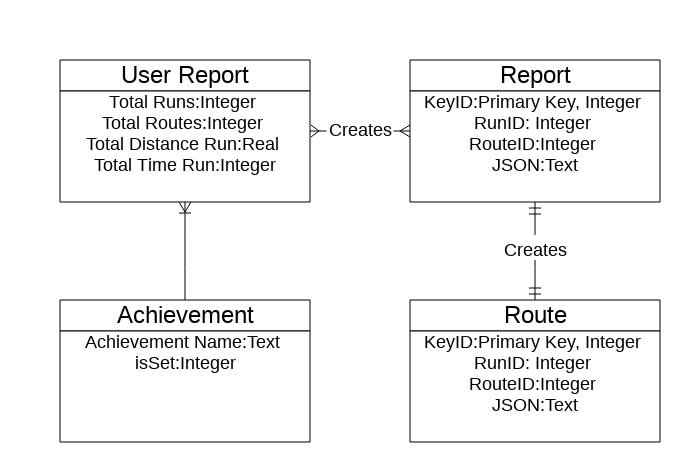
\includegraphics[width=\paperwidth]{westER.png}}
    \end{center}
    \caption{Statistics system ER: Local SQLite Database}
    \label{fig:my_label}
\end{figure}

\subsubsection{Statistics Subsystem Testing}

\paragraph{Introduciton}
Our plan for testing the Statistics subsystem has been divided into three separate phases, which are listed and described in more detail in their own subsections below. These have been divdided into separate parts based upon the domains involved in each part. This is partly due to the issue of the data being passed through two different systems, one being a server the other being a mobile device. This also allows for testing to build off of one another.

\paragraph{Test Plan Parts}
\begin{enumerate}
\item Generating Reports
\item Auditing Reports and Delivery
\item Parsing and Presenting Reports
\end{enumerate}


\paragraph{Testing Phase: Generating Reports}
To test the functionality of this subsystem on the server we have designed three test cases and are currently planning to begin by testing them against using simulated route data to test the functionality these three cases are listed below and have a section that will follow describing them in more detail. After all test cases have passed using simulated data the subsystem will be tested against rotue data generated by our application using the same tests.

\subparagraph{Test Cases}
\begin{itemize}
\item TC-01 Generate Basic Route Report
  \subitem Requirements Fullfilled:
  \begin{enumerate}
    \item System can generate a basic report by using user generated data
    \item The system will use collected geospatial data and user demographic information to present analysis of the user’s performance.
    \item The system will generate a report after a run detailing the user’s performance with comparisons of previous runs.
  \end{enumerate}
\item TC-02 Generate Total Route Report
  \subitem Requirements Fullfilled:
  \begin{enumerate}
    \item System can generate a total report by using user generated data
    \item The system will use collected geospatial data and user demographic information to present analysis of the user’s performance.
    \item The system will take user data and generate leaderboards for heavily used routes incertain areas, in order to allow users to compete for bragging rights on those routes.
    \item The system will generate a report after a run detailing the user’s performance with comparisons of previous runs.
  \end{enumerate}
\item TC-03 Generate Full User Report
  \subitem Requirements Fullfilled:
  \begin{enumerate}
    \item System can generate a complete user report by using user generated data
    \item The system will use collected geospatial data and user demographic information to present analysis of the user’s performance.
    \item The system will take user data and generate leaderboards for heavily used routes incertain areas, in order to allow users to compete for bragging rights on those routes.
    \item The system will generate a report after a run detailing the user’s performance with comparisons of previous runs.
  \end{enumerate}
\end{itemize}

\subparagraph{TC-01 Generate Basic Route Report}
This test case will involve simply taking a user route data from their most recent run and their best run of the same route. It will then compare the two after performing statistical analysis to derive some basic performance data from. The resulting analysis will then be used to create an object derived from the base Report class. The Report derived object will then call the audit function to ensure all fields contain valid format and content.

\subparagraph{TC-02 Generate Total Route Report}
This test case will involve simply taking a user route data from their most recent run and all of their previous runs of that route. It will then compare them after performing statistical analysis to derive a more detailed set of performance data. The resulting analysis will then be used to create an object derived from the base Report class. The Report derived object will then call the audit function to ensure all fields contain valid format and content.

\subparagraph{TC-03 Generate Full User Report}
This test case will involve taking all route and usage data for a user and analyzing it to give that user a detailed performance and usage analysis. This analysis will then be stored in a Report derived object which will then be audited to ensure all fields contain valid format and content.

\paragraph{Testing Phase: Auditing Reports and Delivery}
This next part will be testing the functionality of auditing a report and delivering the report to the user's device. The first part of this test, auditing of the report, is necessary to ensure that the user is being given report data that is valid. Any inconsistencies will result in misleading data or issues with plotting graphs, so it is essential for reports to be complete and contain valid data and types in their repsective fields. The second part will be to ensure that the report data can be sent to the user's device in a format that their device will be able to extract all the report data from. As the reports are generated using Python and the language of the device we have been developing our application on executing Java, this will be an important test.

\subparagraph{Test Cases}
\begin{itemize}
\item TC-04 Auditing Reports
  \subitem Requirements Fullfilled:
  \begin{enumerate}
    \item Ensure reports are properly formatted before delivery
    \item Ensure all report fields contain valid data
    \item The system must generate reports that should be easily readable and detailed while avoiding being confusing to users.
  \end{enumerate}
\item TC-05 Delivering Reports
  \subitem Requirements Fullfilled:
  \begin{enumerate}
    \item Ensure reports objects can be converted to Java objects
    \item Ensures that report can be delivered to the user's device
    \item The system must generate reports that should be easily readable and detailed while avoiding being confusing to users.
    \item The system will generate a report after a run detailing the user’s performance with comparisons of previous runs.
  \end{enumerate}
\end{itemize}

\subparagraph{TC-04 Auditing Reports}
This test case will involve taking reports that have been generated by the system and auditing them. The test will involve taking reports and formatting them into a appropriate data type, likely a string, for delivery to our user's device. Then it will then audit the report by checking to make sure taht all the fields that were in the Report object are in the object. We will begin the testing process by attempting this by using valid reports, reports with all their fields filled, then on invalid reports, reports missing one or more fields or has invalid fields.

\subparagraph{TC-05 Delivering Reports}
This part of this testing phase will involve taking the data type we generated and converting it to a Java equivalent object. Our first test will begin by reading in files containing the report data from storage on the device and converting them into their equivalent Java objects. We will then move to testing when report data is delivered by sending them through the server to client devices.

\paragraph{Testing Phase: Presenting Report Data}
This final phase of testing will involve taking the user reports and processing them for presentation to the user. This will involve generating graphs and listing the report data for the user.

\subparagraph{Test Cases}
\begin{itemize}
\item TC-06 Presenting Report Data
  \subitem Requirements Fullfilled:
  \begin{enumerate}
    \item Display report data to the user
    \item Give user the visual aids and an interface to interact with report
    \item The system must generate reports that should be easily readable and detailed while avoiding being confusing to users.
    \item The system will generate a report after a run detailing the user’s performance with comparisons of previous runs.
  \end{enumerate}

\end{itemize}

\subsubsection{Statistics Subsystem Code}
\paragraph{ReportFactory Code}
This is a snippet below is of the ReportFactory class which will be used to generate reports for a user when delivered a ReportRequest object. This class is the factory portion of our implementation of the factory method design pattern. It will generate a report of the requested type at runtime for a user.
\begin{lstlisting}[language=Python]
import report as rep;
import json;
import numpy as np;
import statistics as stats;
from geopy.distance import vincenty;

class ReportFactory:
    def generate_report(self, request):
        if request.report_type == rep.report_type.basic_report:
            return self.doBasicReport(request.userid, request.routeid);
        elif report_request.report_type == rep.report_type.total_report:
            return self.doTotalReport(request.userid, request.routeid);
        elif report_request.report_type == rep.report_type.full_report:
            return self.doFullReport(request.userid, request.routeid);
        return None;

    def doTotalReport(self, uid, rid):
        #code here...

    def doBasicReport(self, uid, rid):
        #code here...

    def doFullReport(self, uid, rid):
        #code here...
\end{lstlisting}

\paragraph{Report Class Code}
This is code snippet below is for the Python Report class. It is the base class from which all of our report types inherit from.
\begin{lstlisting}[language=Python]
class report:
    def __init__(self, uid, rid, s_t_plots, pace_speed, avgSpd,
    medSpd, maxSpd, currTime, calories_burned):
        self.userid = uid;
        self.routeid = rid;
        self.s_t_plotsx = s_t_plots;
        self.pace_speed = pace_speed;
        self.avgSpeed = avgSpd;
        self.medSpeed = medSpd;
        self.maxSpeed = maxSpd;

    def audit(self):
        return true;

    def sendToDatabase(self):
        return "";

    def sendToUser(self):
        return str(self.userid) + "," + str(self.routeid) + "," + ...;
\end{lstlisting}

\subsubsection{System Conversion and Implementation}
In the process of implementing the Statistics subsystem there was some changes to the system. One of these was to implement the report factory that was the primary part of the system on the android device rather than on the server. This change resulted in the subsytem to have to be coded in Java and utilize several features built in to the android system libraries.

It has als resulted in the addition of another feature to this subsystem, managing the local database on the android device. It was originally part of the Geolocaton subsystem until the redesign of this system required access to it. When it was migrated to the Statistics subsystem it was significantly expanded and additional features were added to handle the demands of both Statistics and the Geolocation subsystems as well as allow better integration with the other subsystems. The additional features required for the Statistics subsystem were to store basic and user reports. The Social and User subsystems required access to these reports to implement some of the features of offered by them.

\subsubsection{Design Alternatives}
We considered two different designs for this subsystem. One approach, the original, was to design and implement this subsystem on the server using Python. The second approach, was to implement the subsystem on the android device using Java. 
\paragraph{First Design Alternative}
The original approach was to integrate the subsystem on the server to be called when data for a route was being saved to the server's database. The subsystem would have called during the saving to create a report and then save the report to the server's database as well. The report would be saved for future requests. The subsystem was going to be implemented using a combination of the Factory Method and the Builder design patterns.
\paragraph{Second Design Alternative}
The second approach, which we decided to implement, was to implement the system on the android device. The system was implemented in very much the same manner as the original, however the reports were generated and stored on the android device's local SQLite database. This approach offered easier access and better security for the User's route data. It also made it easier for the Statistics subsystem to be intergrated with the other subsystem. 

%======================================================================

\subsection{Geolocation Collection and Plotting - Johnny Bragg}
This sub-system, referred to as the Geolocation sub-system, will manage the collection, plotting, and storage of geospatial data that will comprise routes traversed by the user. This data will include: WGS 1984 Latitude and Longitude coordinates, expressed in degrees, minutes, and seconds, Elevation as measured in feet, relative time-stamp information in a 24Hr hh:mm:ss format, and additional derived attributes from the aforementioned data, such as speed, direction, etc.

The sub-system will collect data and write it into an standardized JSON format called GeoJSON for use in the statistics sub-system and storage in the database. Route data will also be accessible by other systems as needed whenever a mapped route needs to be displayed. Additionally, the sub-system will employ two main UI fragments. The first UI fragment will allow a user to track their path as it appears on a web service provided background map in approximately real-time. The second UI will provide a more data oriented synopsis of the user’s current speed, elevation, and coordinates, and will be accessed using a slide up panel visible during data collection. User’s will have the option of exporting data in a comma delimited format for personal use. Other information may be included as the project is revised. The Geolocation sub-system will transmit data to the database back-end for storage and store a local copy of the user's route data on a SQLite database instance on the device to ensure functionality is retained when the User loses service. The DeviceDBHandler class will handle setup and interaction with the database on the device and will synchronize with the external database when needed.

Sending and Receiving of Route information To and From the database server is accomplished by extending Java's AsyncTask\cite{g_AsyncTask} class to two new classes: FetchData and SendData and an interface in each class. An implementation of FetchData was found online and modified to handle POST requests as well as GETs.\cite{g_asyncget} The main map activity will implement interfaces for both classes to avoid blocking the UI during requests and while the application awaits a response from the server.

\subsubsection{User Requirements}
\begin{itemize}
    \item System will use device sensors to record GPS data in a Latitude/Longitude format.
    \item System will use device sensors to record user elevation.
    \item System will plot Geolocation data against a Google provided background map.
    \item System will record relative time stamps to use in calculation of speed and direction.
    \item System will display user activity duration, speed, distance, current elevation, and coordinates during data collection.
    \item System will display user routes clearly and in real-time as data is being collected.
    \item System will allow the user to save individual routes to a comma-delimited file for personal use.
    \item System will display traversed routes in the User's immediate vicinity.
    \item System will allow a user to tap on a route to retrieve and view information associated with that route.
    \item System will store a user’s routes in a particular format for use in Pathway.
    \item System will maintain a local device database to store a user's route data.
    \item System will be available as long as a persistent data connection is allowed.
    \item System will be made available in a limited capacity with reduced accuracy and no map service while no data connection exists.
    \item System will accurately and precisely locate the user’s position within an acceptable margin of error, allowing for a larger margin where service is weak or none exists.
\end{itemize}

\subsubsection{Process}
The system will be completed an tested over the course of the Fall 2017 semester, with regular updates to follow.

\subsubsection{Domain Analysis}
\paragraph{Introduction}
This document conveys a brief overview of GPS based data plotting and collection as is commonly used in mapping applications. This is a well-established domain, with many existing applications employing mapping systems to some degree.

\paragraph{Extensions}
Possible extensions may include extension of data review to a website interface. Functionality beyond the mapping capabilities is unnecessary and will be constrained to only those updates required to maintain functionality as updates occur to the API or updates to correct any bugs discovered in operation.

\paragraph{General Domain Knowledge}
\begin{itemize}
    \item  Most mobile devices are GPS capable.
    \item Most mobile devices include sensors to count steps and track speed.
    \item Many people who walk/run for fitness maintain some records of times/speeds to track progress.
    \item Fewer people maintain information regarding where they perform fitness activities outside of a gym or similar facility.
    \item Generally, fitness programs are more successful if personal improvement is apparent. (Times noticeably decrease, weight is lost, strength measurably improves, etc.)
    \item Fitness journals and programs that monitor progress help people stick with a program.
\end{itemize}

\paragraph{Clients and Users}
The primary clients of the mapping sub-system will be the other sub-systems comprising Pathway, who will depend on the mapping sub-system to collect and store the data used in those sub-systems. Users of Pathway will interact with the Geolocation sub-system to initiate data collection, describe routes, and save completed routes.

\paragraph{The Environment}
All actors in this process will need access to a GPS enabled tablet or cell phone running Android v5 or later.  The final product will require an active data connection to write and retrieve data from the database and to retrieve base-map information from Google servers.

\paragraph{Tasks and Procedures}
\begin{itemize}
\item Finding user location using GPS: The sensors perform an initial ping of satellite locations to establish a start location.
\item GPS accuracy is limited by device and location constraints. Specifically, mountainous or very built-up urban areas may produce signal “bouncing”, causing the GPS to lose accuracy.
\item Subsequent positions are found by pinging the sensors every x seconds.
\item GPS location may be supplemented using triangulation through wi-fi networks and cell towers.
\item Recording the current user position: The information collected by the device sensors is in the form of Lat/Long coordinates and an elevation value, typically measured in feet.
\item Storing user location over a period of time: User information (Lat/Long, Elev, etc.) is stored in a text file or data structure to allow review at a later date.
\item Additional functions may be performed using the data collected in the above methods. This may include: Plotting of data in real-time.
\item Calculation of derived information that may be useful to the user. This includes: speed, direction.
\end{itemize}

\paragraph{Competing Software}
Our research has discovered that many applications incorporate mapping information into their functionality. Due to the widespread usefulness of the system, the general nature of the software, and the fact that the api used is offered free of charge, it can be argued that there are no competitors. Similar software products exist but are marketed on their utility either outside of mapping or by some unique feature in tandem with mapping.

\paragraph{Domain Similarities}
Mapping applications like the one we envision are common, and the usefulness of geographic data is apparent in many fields and industries. There is no shortage of similar systems available for use, so documentation is both plentiful and current. Due to the general nature of this sub-system, we are not concerned that any similarities would constitute a duplication of an existing system. The widespread usage of similar systems does however provide us with a wealth of information to be used towards development of our own system.

\subsubsection{System Analysis}
\paragraph{Introduction}
The geolocation subsystem is relatively isolated from other subsystem within the Pathway project. The primary interaction between the geolocation
subsystem and other subsystems will be in the passing of an instance of the Route class, which will extend functionality of the JSONObject datatype. The mapping functionality of the subsystem will be implemented by leveraging existing classes and objects within
the Google Maps API and as such will not require extensive coding to achieve the desired functionality and layout.
This functionality would include map display, panning, zoom, and drawing of features on the map.


\paragraph{Algorithms}
To implement the route comparison feature, we have reviewed two algorithms that break the problem down into a comparison of ordered sets of pairs:
Hausdorff distance and Fréchet distance. 
The Hausdorff measures how far two subsets of a metric are from each other. \cite{g_hausdorff}Between these two algorithms, there is a tradeoff of complexity versus versatility,
which can be summarized as below, with included pseudocode for Hausdorff.

\begin{algorithm}[h]
\SetAlgoLined
$h \gets 0$\\
\For{point $a_i$ in $A$}{
    $shortest \gets \infty$

    \For{point $b_j$ in $B$}{
        $d_{ij} \gets d(a_i,b_j)$\\
        \If{$d_{ij} \< shortest$}{
            $shortest \gets d_{ij}$\\
        }
    }
    \If{$shortest \> h$}{
        $h \gets shortest$
    }
}
\caption{Hausdorff distance for ordered sets of coordinate pairs.}
\end{algorithm}

The Fréchet distance is a measure of similarity between curves that takes into account the location and ordering of the points along the curves.\cite{g_frechet} It is more complex and harder to implement, but generally more versatile and supports backtracking. Pseudo code omitted due to complexity.

At this stage of the project, we plan to implement both algorithms and compare their accuracy against a series of test cases designed to assess the correctness and flexibility of each algorithm.

Additionally, we have created a basic route comparison algorithm that will run first, saving computation time. The simple version of the algorithm takes two Routes as input and recursively compares start and end points of line segments within the route up to five recursions, beginning with the total route.
\newline Note: n is the last element in the Route.\newline

\begin{algorithm}[H]
\SetAlgoLined
\If{ \(counter < 10 \)}{
\If{start $Route1$ near start $Route2$ AND 
    end $Route1$ near end $Route2$}{
    $counter \gets $counter + 1\\
    $k \gets $floor(n/2)$\\
    basicCompare($Route1[0:k]$, $Route2[0:k]$, $counter$)\\
    basicCompare($Route1[k+1:n]$, $Route2[k+1:n]$, $counter)\\
    }
}
\caption{basicCompare(Route 1, Route 2, counter)}
\end{algorithm}

\pagebreak
\paragraph{Tool Selection}
Due to the reliance of the geolocation system on an existing API, our tool selection will include the Google Maps API\cite{G_API_Maps}, Google Elevation API\cite{g_API_Elev}, and code provided by the Google Maps Utility Library\cite{g_Util_Map}, and the development tools and language that were selected for the project as a whole. The system will be coded entirely in Java, primarily using the Google Maps API and leveraging Android Studio to more easily create the application layout. A SQLite database will be created on the local device to store information until a connection can be established with the Pathway server. The local database will closely mimic the structure of the external server. The above mentioned algorithms will be coded as methods within the Route class, which will store all representations of route data. Currently, the geolocation system design will employ at least 5 classes, with additional classes likely being added in the course of development. These classes may be altered or replaced as research into the API continues.

\paragraph{Use Cases}

\begin{figure}[H]
    \centering
    \begin{center}
        \makebox[\textwidth]{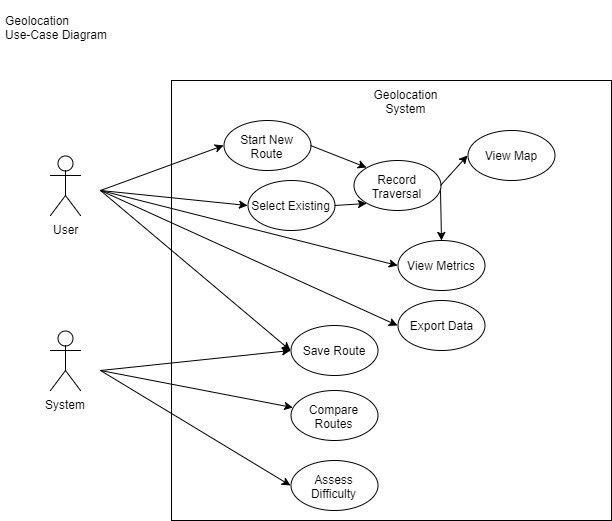
\includegraphics[width=0.8\paperwidth]{braggUseCaseDaig.jpg}}
    \end{center}
    \caption{Geographic system use case diagram}
    \label{fig:my_label}
\end{figure}
% \begin{figure}
%     \centering
%     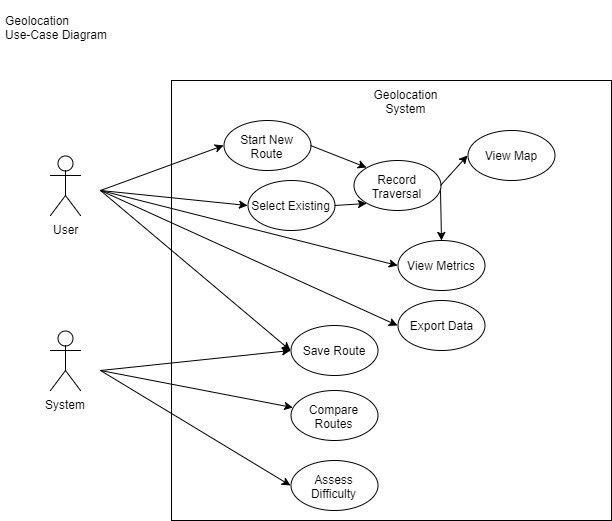
\includegraphics[width=\textwidth]{braggUseCaseDaig.jpg}
%     \caption{Geolocation use case diagram}
%     \label{fig:my_label}
% \end{figure}
\pagebreak
\begin{enumerate}
\item User starts a new route.
    \begin{enumerate}
        \item Actors: User
        \item Preconditions: System is idle and no existing route is selected.
        \item Flow:
            \begin{enumerate}
                \item User presses start route.
                \item System prompts user to select activity.
                \item Route begins recording.
            \end{enumerate}
        \item Postcondition: User is recording a route.
    \end{enumerate}
\item User starts an existing route.
    \begin{enumerate}
        \item Actors: User
        \item Preconditions: User has selected an existing route from the map and is currently near the start of the route.
        \item Flow:
            \begin{enumerate}
                \item User presses start existing route.
                \item Route begins recording.
            \end{enumerate}
        \item Postcondition: User is recording a new traversal of existing route
    \end{enumerate}
\item User completes and saves a traversal.
    \begin{enumerate}
        \item Actors: User and System.
        \item Preconditions: User is currently recording a traversal.
        \item Flow One: New Route.
            \begin{enumerate}
            \item User presses Stop and is prompted to name and save.
            \item System stores Route information in database.
            \item System returns to idle.
            \end{enumerate}
        \item Flow Two: Existing Route.
            \begin{enumerate}
            \item User presses Stop and is prompted to name and save.
            \item System verifies that traversal matches the selected Route.
            \item System stores Route information in database.
            \item System returns to idle.
            \end{enumerate}
        \item Postconditions: System is idle.
    \end{enumerate}
\item User wants to view track information.
    \begin{enumerate}
        \item Actors: User and System.
        \item Preconditions: Two Cases
            \begin{enumerate}
            \item User has selected an existing map and is not currently recording.
            \item User is currently recording a new or existing.
            \end{enumerate}
        \item Flow:
            \begin{enumerate}
            \item User presses the info button.
            \item A new view fragment appears to display past and/or current user performance.
            \item User returns to map screen.
            \end{enumerate}
        \item Postconditions: None
    \end{enumerate}
\item User wants to export data.
    \begin{enumerate}
        \item Actors: User, System
        \item Preconditions: User has selected an existing or completed a new or existing route.
        \item Flow:
            \begin{enumerate}
            \item User selects Export.
            \item System prompts user for file destination.
            \item System saves csv onto local device.
            \end{enumerate}
        \item Postconditions: A file exists on the local device.
    \end{enumerate}
\item System wants to compare two routes.
    \begin{enumerate}
        \item Actors: System
        \item Preconditions:
            \begin{enumerate}
            \item Routes have overlapping bounding boxes.
            \item Routes have similar total distances.
            \end{enumerate}
        \item Flow:
            \begin{enumerate}
            \item System checks for preconditions to be true before continuing.
            \item System calculates a similarity score using two routes as input.
            \item System decides if routes are similar based on score.
            \item If similar, store route information using ID of original track.
            \item If not, store new route information.
            \end{enumerate}
        \item Postconditions: Route is stored in database.
    \end{enumerate}
\item System wants to determine difficulty of Route.
    \begin{enumerate}
        \item Actors: System
        \item Preconditions: Route has been traversed and has not yet been saved.
        \item Flow:
            \begin{enumerate}
            \item System uses a naive method to assign difficulty rating, based on distance.
            \item System uses a naive method to assign difficulty rating, based on length of route and elevation variability, which will be defined as the difference between maximum and minimum elevations.
            \end{enumerate}
        \item Postconditions: Route has an estimated difficulty assigned.
    \end{enumerate}
\end{enumerate}

\paragraph{Classes}
Classes, their interaction, and the general flow of the subsystem are depicted in the following diagrams.

\begin{figure}[H]
    \centering
    \begin{center}
        \makebox[\textwidth]{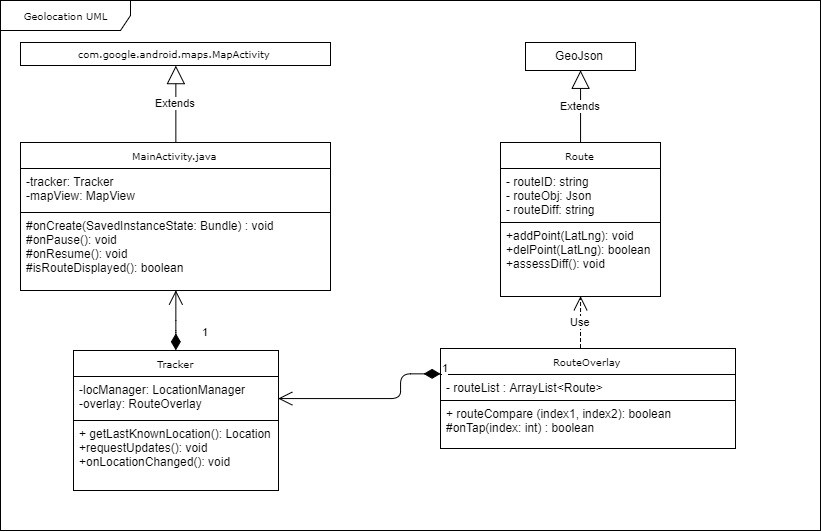
\includegraphics[width=0.8\paperwidth]{braggUML.jpg}}
    \end{center}
    \caption{Geolocation UML diagram}
    \label{fig:my_label}
\end{figure}
% \begin{figure}[H]
%     \centering
%     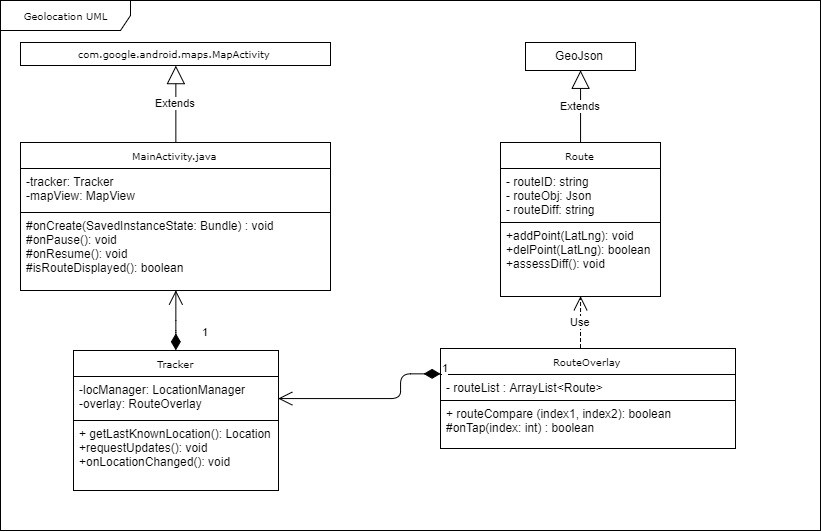
\includegraphics[width=\textwidth]{braggUML.jpg}
%     \caption{Geolocation UML diagram}
%     \label{fig:my_label}
% \end{figure}

The system will be comprised of 5 classes, aside from strictly UI classes. Classes marked with * are classes from the Maps API. The MainActivity will maintain instances of the Location* class and GoogleMap* class, which will be used to retrieve user location and display the map, respectively. The Route class will handle storage and retrieval of information in conjunction with Google's Polyline class. Each Route object will contain identifying information, location data, and additional attributes as necessary. Routes will be retrieved from the database based on current geographic location. Route will inherit from the JSONObject datatype and will follow geojson conventions as described by Butler et al \cite{g_geojson_std}, allowing it to store geolocation information in a standard format.

\begin{figure}[H]
    \centering
    \begin{center}
        \makebox[\textwidth]{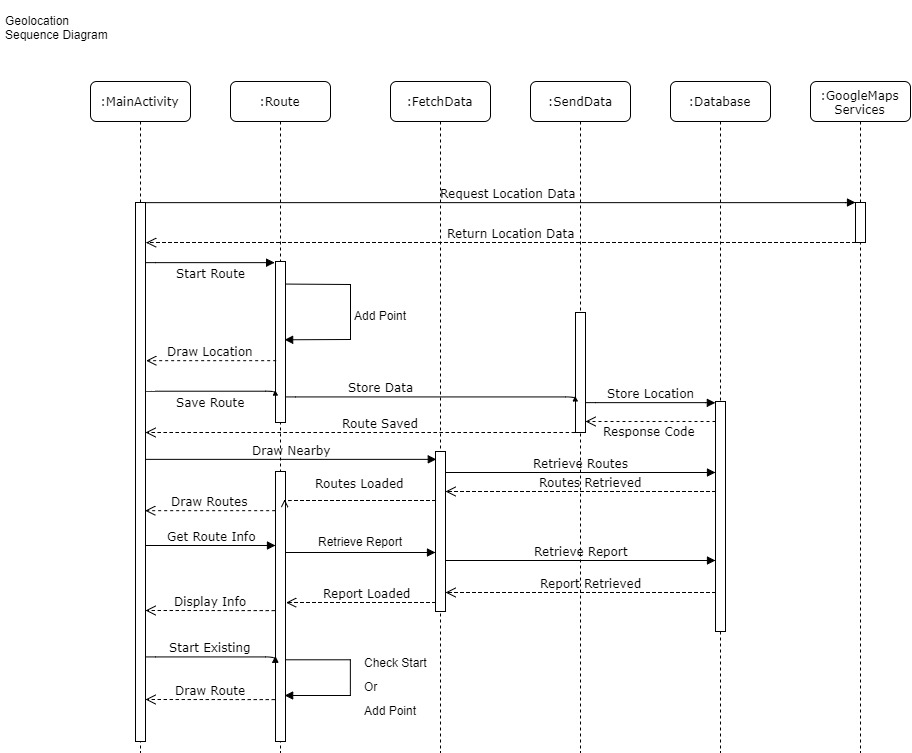
\includegraphics[width=0.8\paperwidth]{braggSEQ.jpg}}
    \end{center}
    \caption{Geolocation sequence diagram}
    \label{fig:my_label}
\end{figure}

% \begin{figure}[H]
%     \centering
%     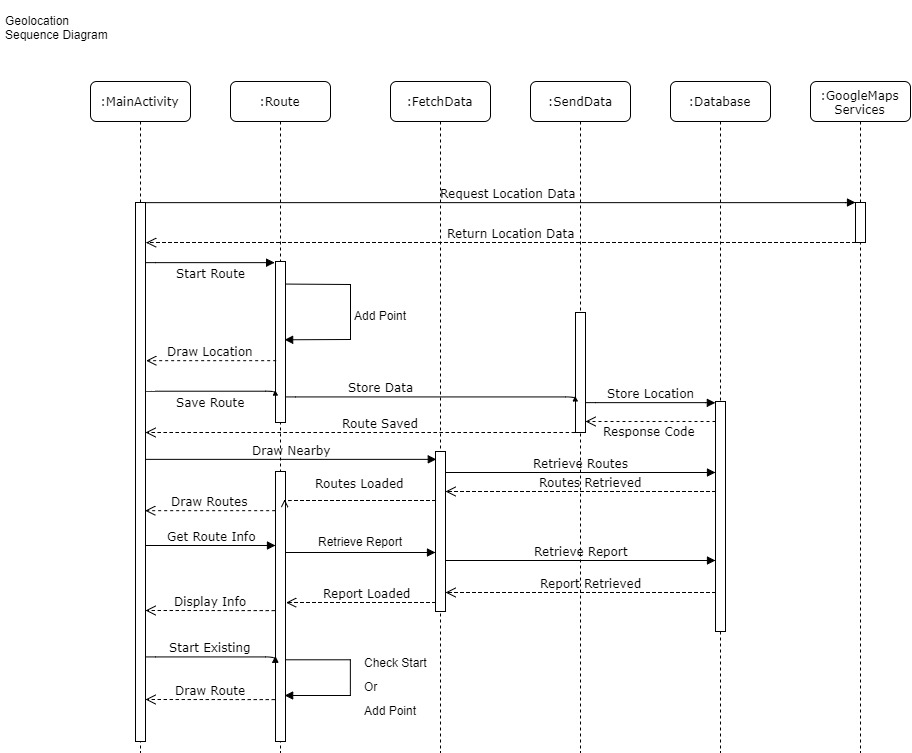
\includegraphics[width=\textwidth]{braggSEQ.jpg}
%     \caption{Geolocation sequence diagram}
%     \label{fig:my_label}
% \end{figure}

\begin{figure}[H]
    \centering
    \begin{center}
        \makebox[\textwidth]{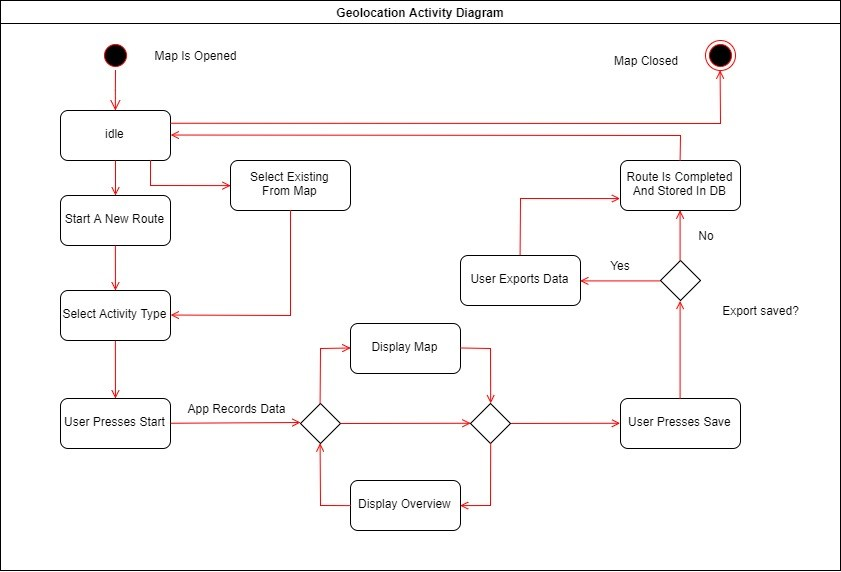
\includegraphics[width=0.8\paperwidth]{braggActivity.jpg}}
    \end{center}
    \caption{Geolocation activity diagram}
    \label{fig:my_label}
\end{figure}

% \begin{figure}[H]
%     \centering
%     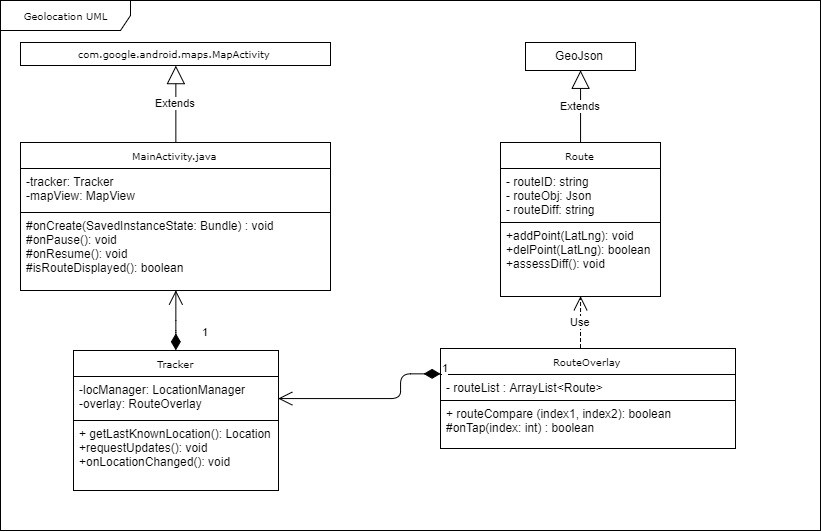
\includegraphics[width=\textwidth]{braggUML.jpg}
%     \caption{Geolocation activity diagram}
%     \label{fig:my_label}
% \end{figure}
%=====================================================

\newpage
\subsection{Testing Plan}
\subsubsection{Test Overview}
In order to test the geolocation functionality of our application, we have derived a series of test cases, corresponding to specific requirements in the User Requirements section of the Geolocation subsystem.
Tests were performed on an emulated Nexus 5 running Android 5.0 and on an LG G3 device running Android 6.0. The primary goal of the tests were to ensure correct operation of GPS sensors and utilization of device location data. The following tests do not comprise an exhaustive list of all tests to be performed and do not satisfy all User Requirements of the Subsystem. Additional tests will be performed as development continues to satisfy all remaining requirements.
Test Cases:
\begin{itemize}
\item TC-01 - Get Device Location
\item TC-02 - Draw User Route
\item TC-03 - Functionality With No Data Access
\end {itemize}
The following terms are used in describing these tests:
\begin{itemize}
\item Camera - Refers to the overhead view within the map frame.
\item MyLocation - Standard Map API control to query for device location.
\end {itemize}

\subsubsection{Test Cases}
\begin {itemize}
\item TC-01: Get Device Location
\subitem Requirement(s) Fulfilled:
\subsubitem System will use device sensors to record GPS data in a Latitude and Longitude format.
\subsubitem System will plot Geolocation data against a Google provided background map.
\subitem Description: The device retrieves the current location and centers the map on that position. For the test, the map begins centered on a marker placed at Sydney Australia. Upon pressing the My Location button in the upper corner, the map is recentered to the current location.
\subitem Precondition: User has logged into Pathway.
\subitem Test Steps:
\subsubitem 1. Application is started.
\subsubitem 2. Press MyLocation Button
\subsubitem 3. Map pans to user.
\subsubitem 3. Observe Results Of Location Change.
\subitem Expected Result: Current Location of the User is shown.
\subitem Actual Result: Map view pans to current location, as shown in Figures 17 and 18.
\subsubitem Additionally, manually moving camera and clicking MyLocation successfully recenters view on the User's location.
\subitem Related Code:
\begin{lstlisting}[
basicstyle=\small
]
public void onMapReady(GoogleMap googleMap) {
    // Add a marker in Sydney, Australia,
    // and move the map's camera to the same location.
    mMap = googleMap;
    LatLng sydney = new LatLng(-33.852, 151.211);
    googleMap.setMapType(GoogleMap.MAP_TYPE_TERRAIN);
    googleMap.addMarker(new MarkerOptions().position(sydney)
    .title("Marker in Sydney"));
    googleMap.moveCamera(CameraUpdateFactory.newLatLng(sydney));
    if (ActivityCompat.checkSelfPermission(this,
    Manifest.permission.ACCESS_FINE_LOCATION)
    != PackageManager.PERMISSION_GRANTED) {

    ActivityCompat.requestPermissions(this,
        new String[]{Manifest.permission.ACCESS_FINE_LOCATION}, 1);
    return;
    }
    googleMap.setOnMyLocationButtonClickListener(this);
    googleMap.setMyLocationEnabled(true);
}
\end{lstlisting}


\item TC-02: Draw User Route
\subitem Requirement(s) Fulfilled:
\subsubitem System will plot Geolocation data against a Google provided background map.
\subsubitem System will display user routes clearly and in real-time as data is being collected.
\subitem Description: Draws the users route on the map as a path is traversed, updating the current position at regular intervals.
\subitem Precondition: User's location has been found, and the Start Button has been pressed. GPS must be enabled.
\subitem Test Steps:
\subsubitem 1. User presses Start
\subsubitem 2. User begins traversing an area.
\subitem Expected Result: Route is drawn on screen.
\subitem Actual Result: Route is successfully drawn on screen. Figures 18 and 19 show traversals in a localized area (roughly 100 ft) and across approximately 4 miles, respectively.
\subitem Related Code:
Code fires when Start button is pressed.
\begin{lstlisting}[
basicstyle=\small
]
public void onStartPressed(View v) {
    if (runState == RunStates.OFF) {
        btnStart.setText("Stop");
        Snackbar.make(v, "Recording...", Snackbar.LENGTH_LONG)
        .setAction("Action", null).show();

        runState = RunStates.RUN;
        PolylineOptions routeOptions = new PolylineOptions()
        .color(Color.RED)
        .width(12)
        .startCap(new RoundCap())
        .endCap(new RoundCap());
        timerRoute.setBase(SystemClock.elapsedRealtime());
        timerRoute.start();
        userRoute = mMap.addPolyline(routeOptions);
        startLocationUpdates();
    }
    else if(runState == RunStates.RUN) {
        btnStart.setText("Start");
        Snackbar.make(v, "Recording Stopped.", Snackbar.LENGTH_LONG)
        .setAction("Action", null).show();

        runState = RunStates.OFF;
        userRoute.remove();
        userRoute = null;
        timerRoute.stop();
        stopLocationUpdates();
    }
}
\end{lstlisting}
Code responsible for adding most recent location to Polyline and displaying on screen.
\begin{lstlisting}[
basicstyle=\small
]
public void onLocationChanged(Location location) {
    lastLoc = new LatLng(
    location.getLatitude(),
    location.getLongitude()
    );
    if (userRoute != null) {
        List<LatLng> points = userRoute.getPoints();
        points.add(lastLoc);
        userRoute.setPoints(points);
    }
    coordMsg = String.format("XY: %s.", lastLoc.toString());
    mMap.animateCamera(CameraUpdateFactory.newLatLng(lastLoc));
    mMap.animateCamera(CameraUpdateFactory.newLatLngZoom(lastLoc, 16));
}
\end{lstlisting}

\item TC-03: Functionality With No Data Access
\subitem Requirement(s) Fulfilled:
\subsubitem System will be available as long as a persistent data connection is allowed.
\subsubitem System will be made available in a limited capacity with reduced accuracy and no map service while no data connection exists.
\subitem Description: The system will make use of GPS sensors when a data connection isn't available. In the event of sudden data loss, the system continues to track and draw User location.
\subitem Precondition: System has a GPS signal and Route is being recorded.
\subitem Test Steps:
\subsubitem 1. User presses Start.
\subsubitem 2. System begins recording with no data connection, or data connection is lost during recording.
\subitem Expected Result: Application continues collecting GPS data and plotting route. Background map will not be available while data is unavailable.
\subitem Actual Result: Route continued to record while data was unavailable (Figures 19 and 20). Quality of data suffered, and was noisy when the User was stationary, due to resolution of GPS sensor, which produced false movement along the route. (Figure 21).
\subitem Related Code: No specific code was needed to ensure this functionality.
\end {itemize}
\subsubsection{Test Case Figures}
\begin{figure}[H]
    \centering
    \begin{center}
        \makebox[\textwidth]{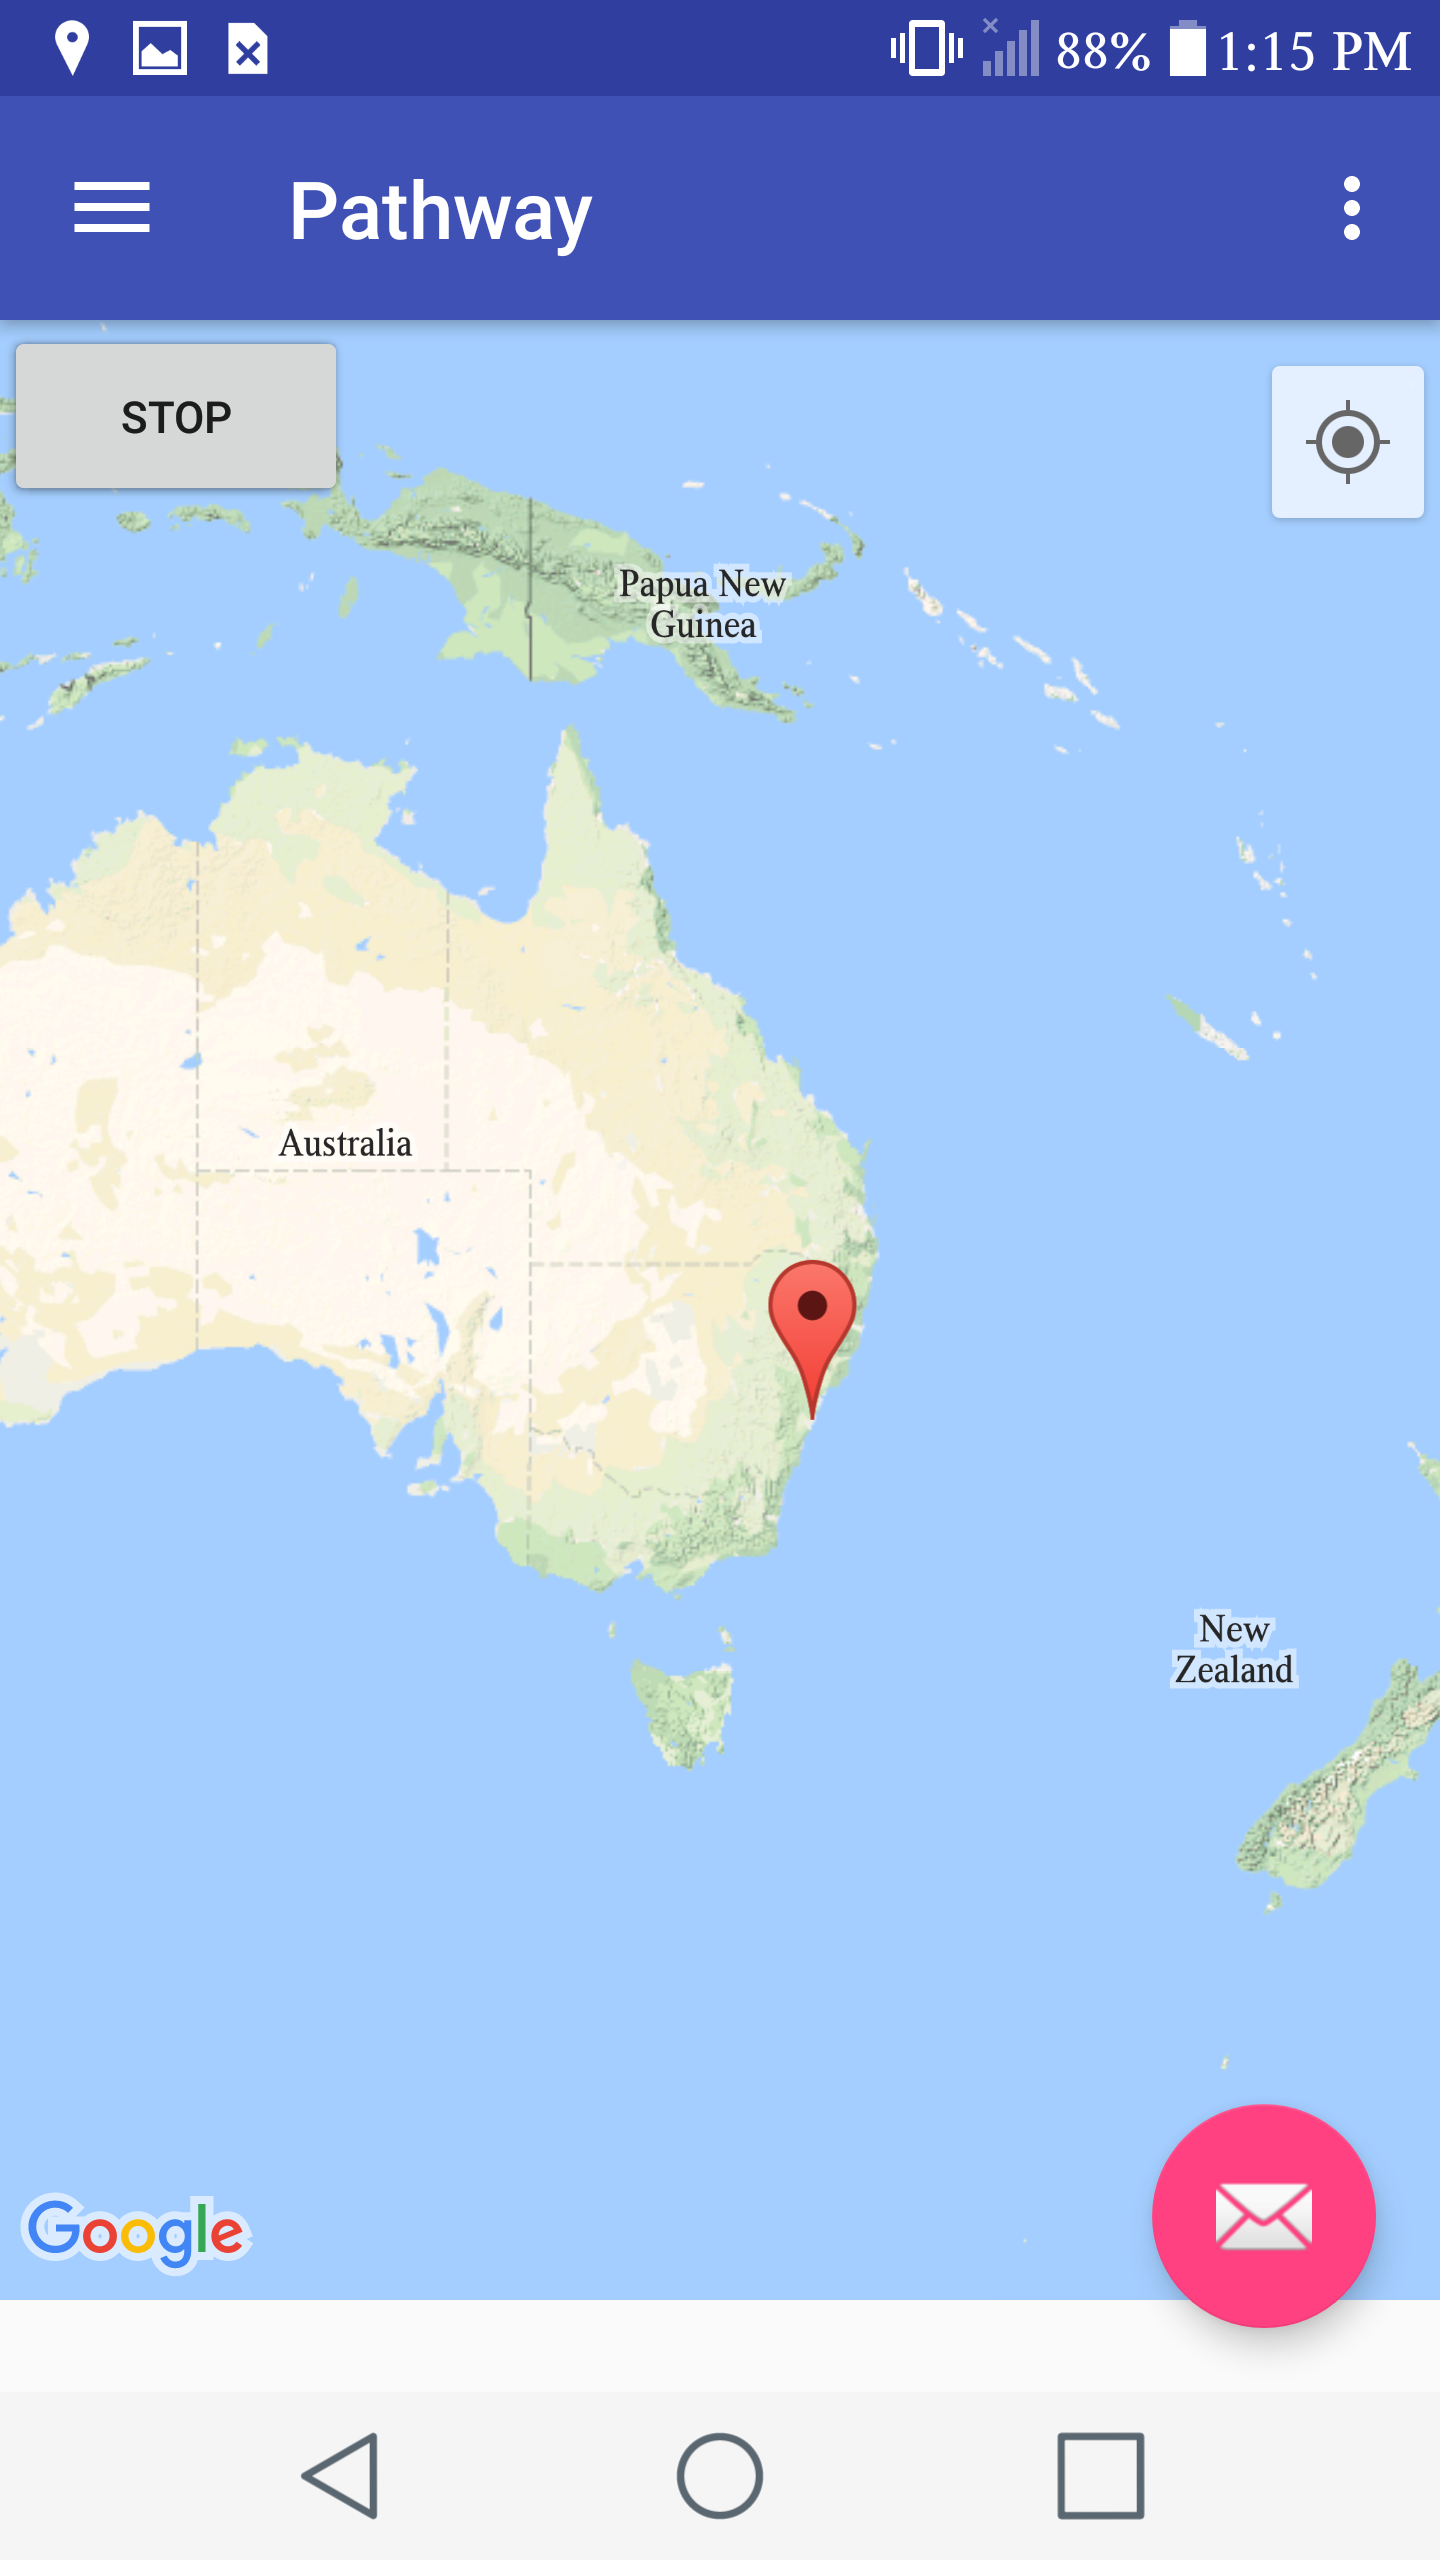
\includegraphics[totalheight=0.40\textheight]{GeoTestDev1.png}}
    \end{center}
    \caption{Initial Location - Sydney, Australia}
    \label{fig:my_label}
\end{figure}

\begin{figure}[H]
    \centering
    \begin{center}
        \makebox[\textwidth]{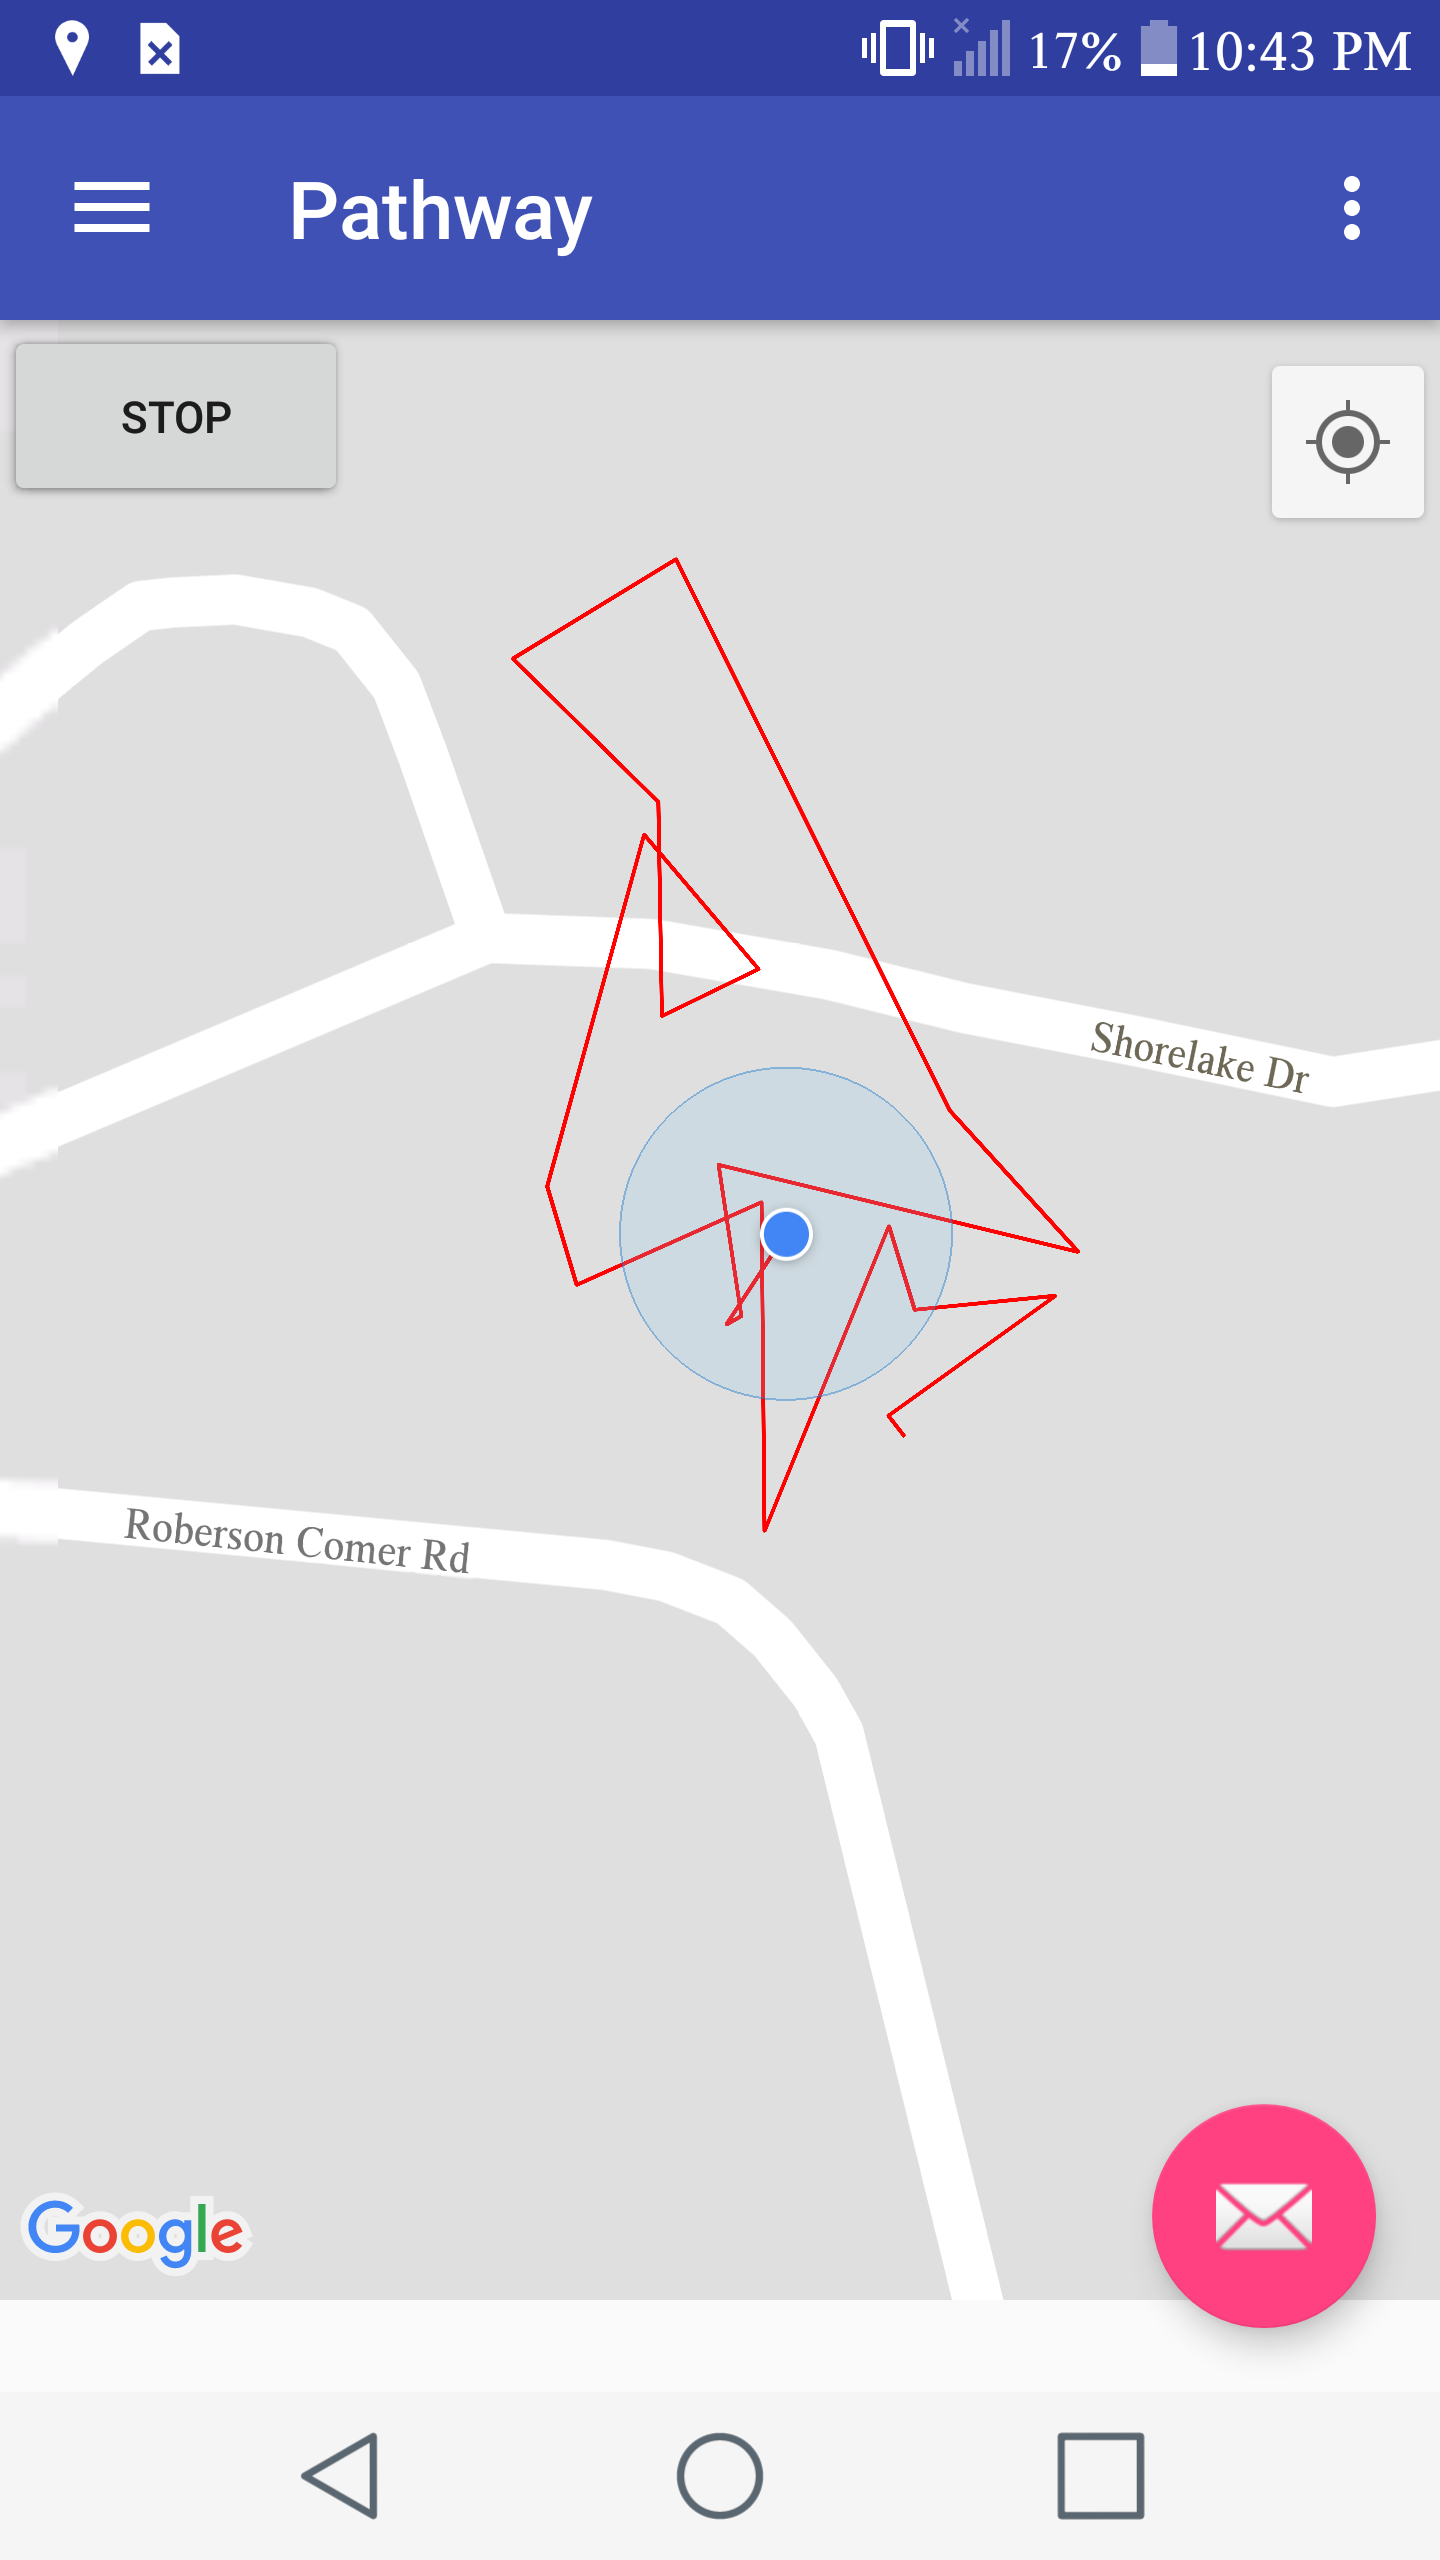
\includegraphics[totalheight=0.4\textheight]{GeoTestDev2.png}}
    \end{center}
    \caption{Current Location - Includes depiction of test route.}
    \label{fig:my_label}
\end{figure}
\begin{figure}[H]
    \centering
    \begin{center}
        \makebox[\textwidth]{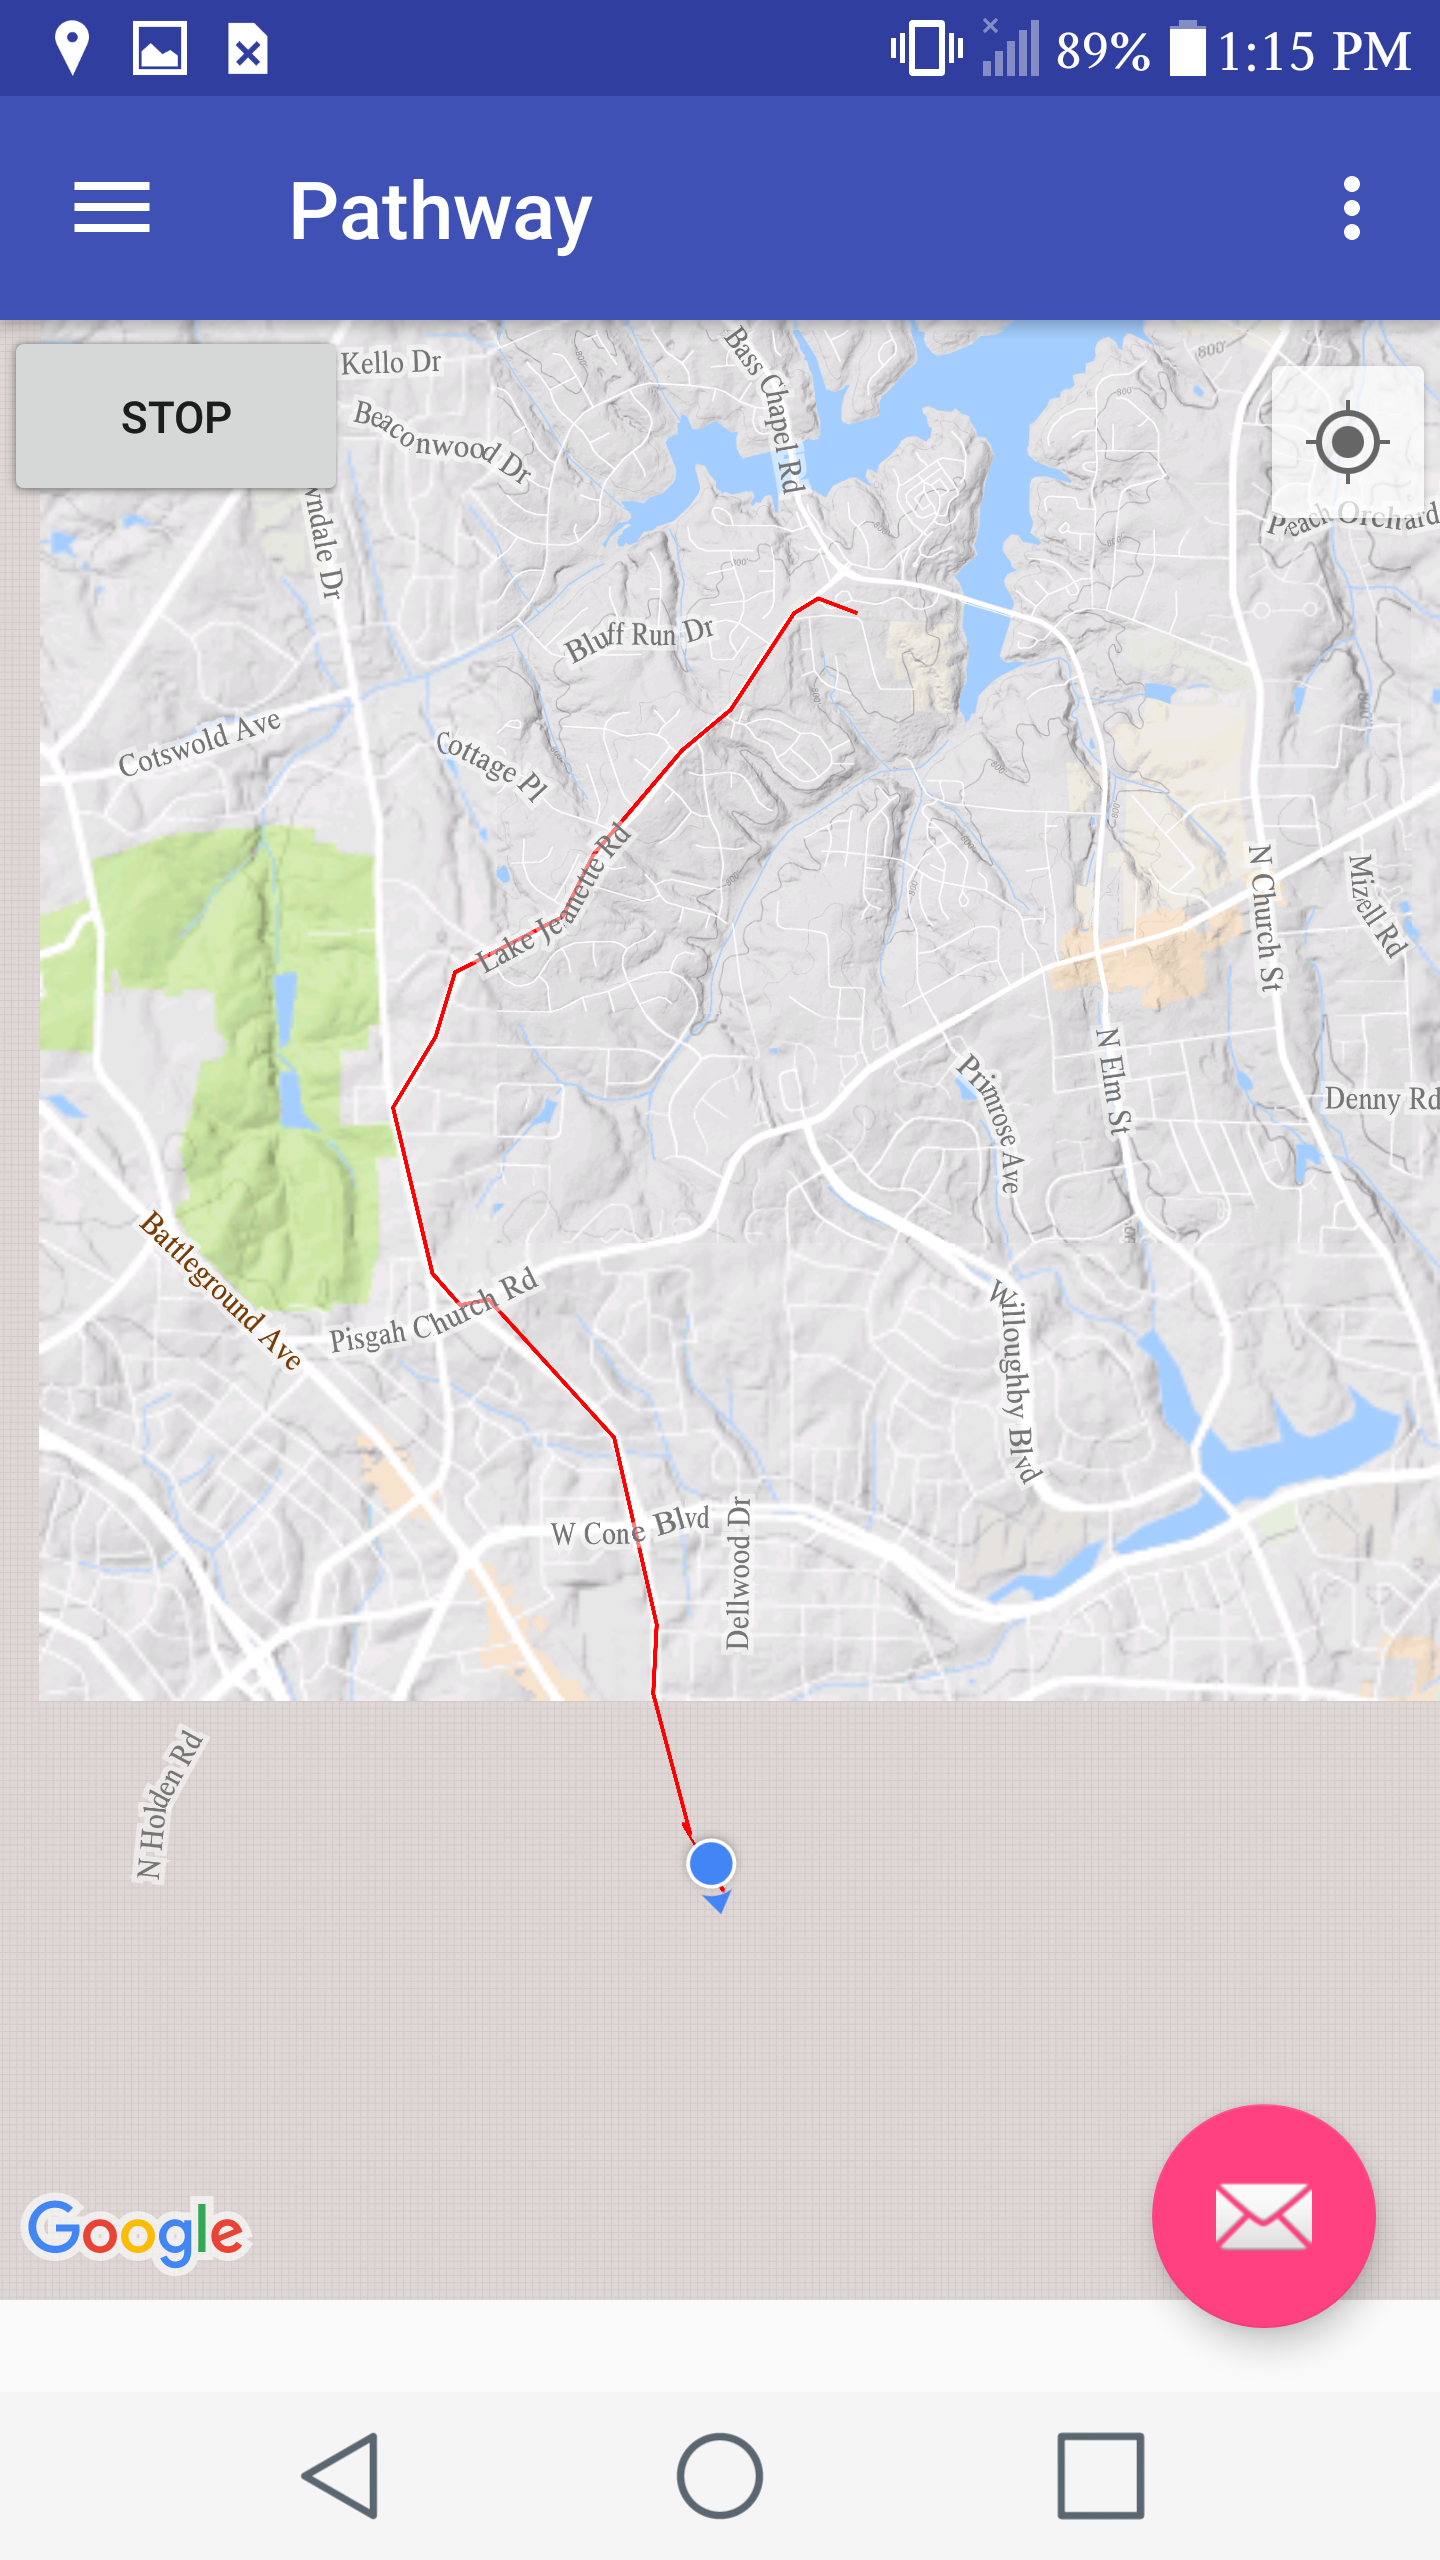
\includegraphics[totalheight=0.4\textheight]{GeoTestNoDataDev1.png}}
    \end{center}
    \caption{Map showing traversal through area after data loss.}
    \label{fig:my_label}
\end{figure}
\begin{figure}[H]
    \centering
    \begin{center}
        \makebox[\textwidth]{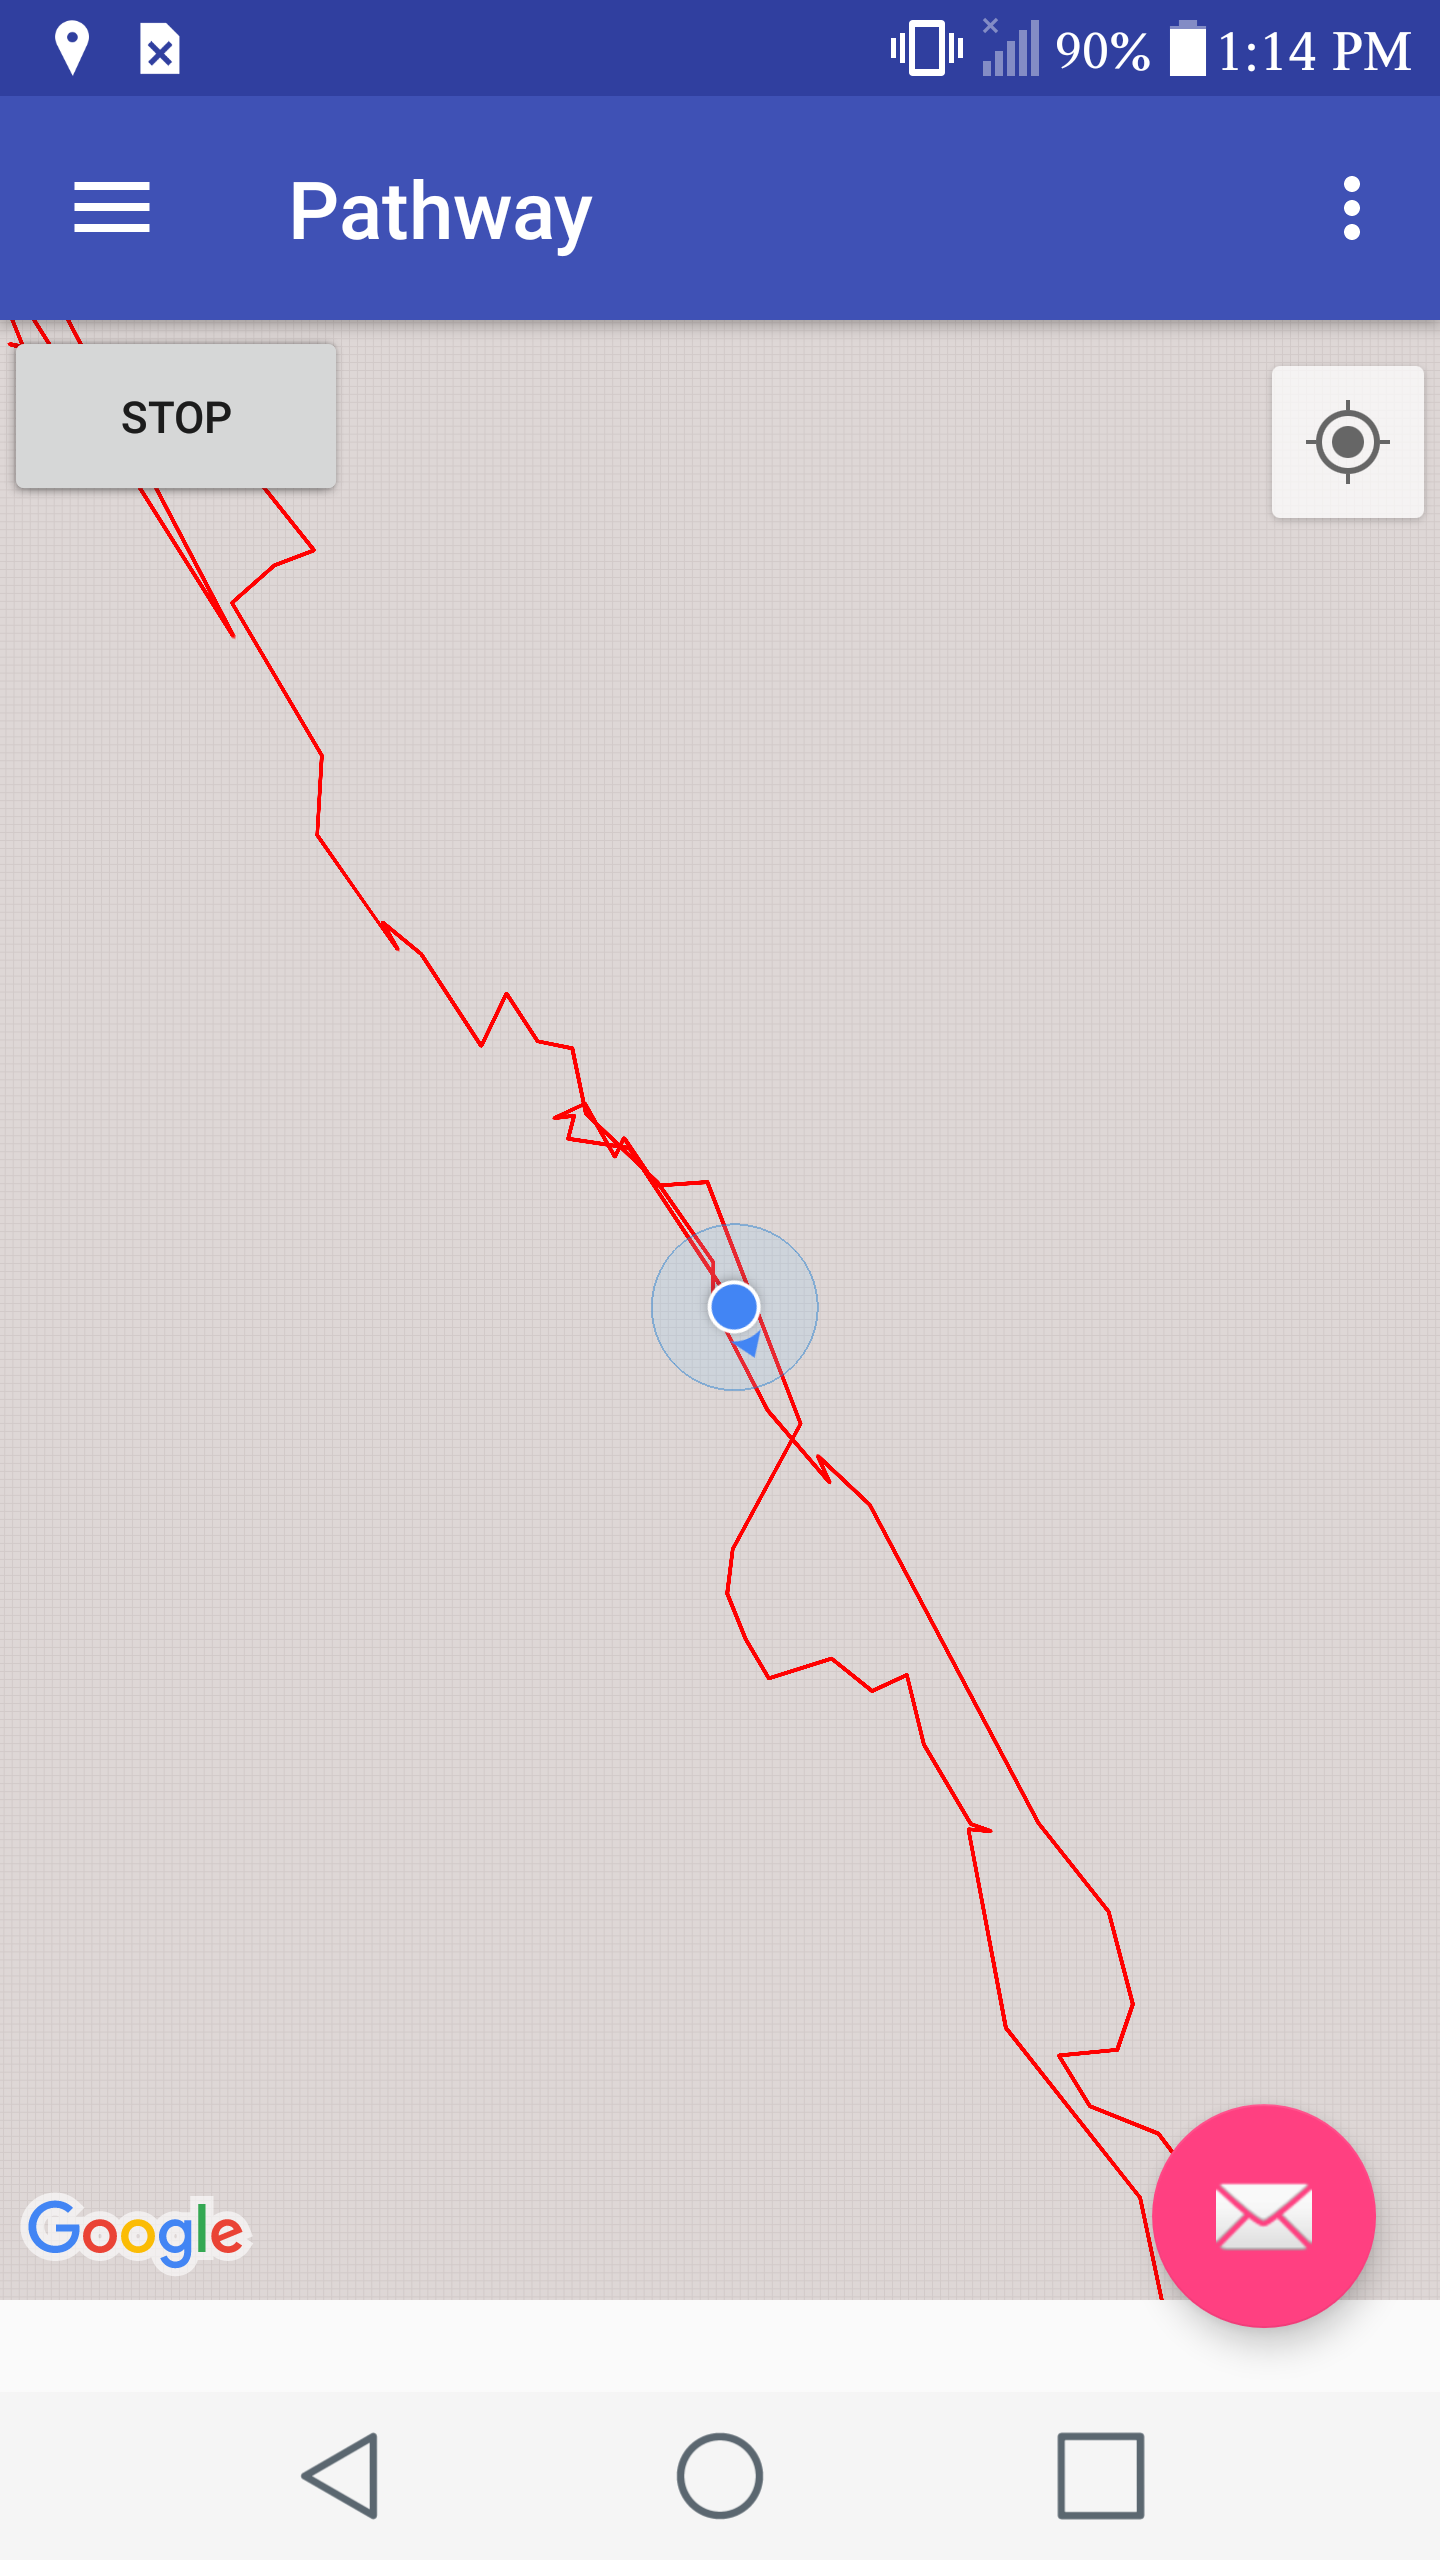
\includegraphics[totalheight=0.4\textheight]{GeoTestNoDataDev2.png}}
    \end{center}
    \caption{Traversed same area several times to show variance along route.}
    \label{fig:my_label}
\end{figure}
\begin{figure}[H]
    \centering
    \begin{center}
        \makebox[\textwidth]{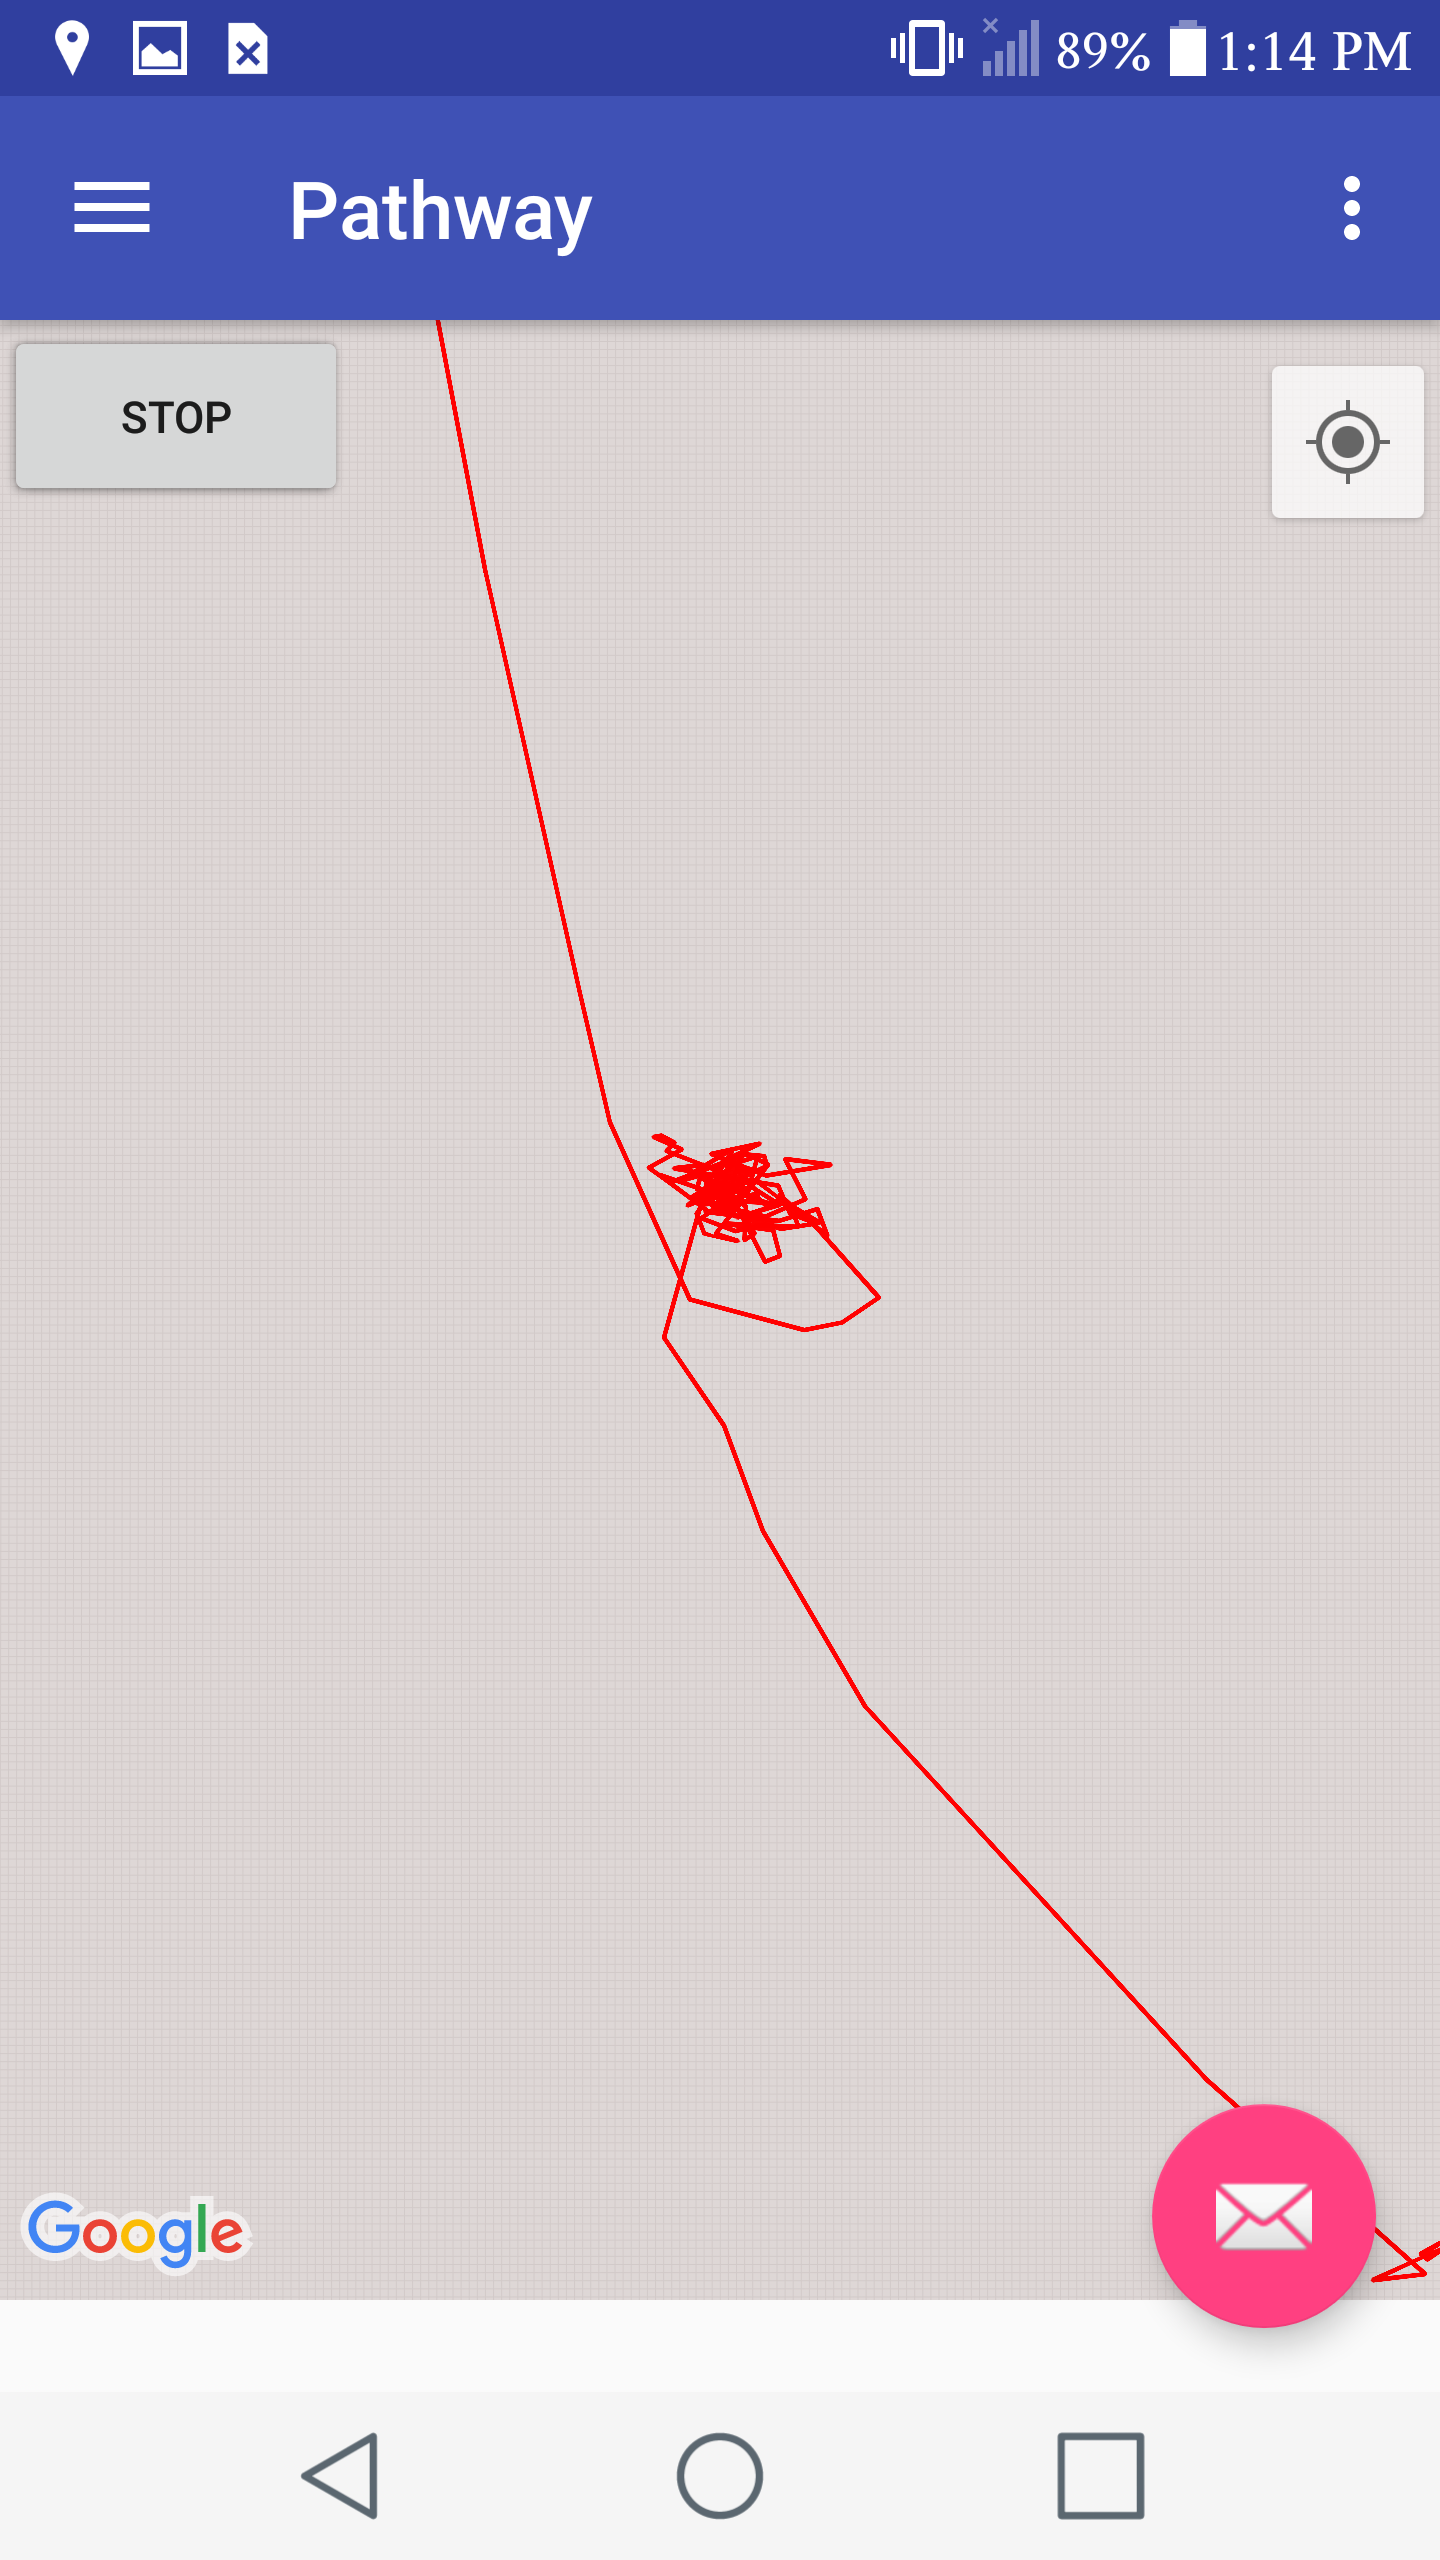
\includegraphics[totalheight=0.4\textheight]{GeoTestNoDataDev3.png}}
    \end{center}
    \caption{"Bunched" data, collected while stationary without data connection. Shows GPS variance.}
    \label{fig:my_label}
\end{figure}

\subsubsection{Test Summary}
Tests performed to ensure accuracy of geolocation on a handheld device were largely successful. Latitude and Longitude values were within expected deviations from actual values as provided by Google Maps each time. While generally accurate, situations where data connection is lost produce less than ideal coordinate values and as such shall be avoided when possible. Prolonged loss of data connection would likely produce unusable data sets, but temporary outages should be able to be handled by the system.
B
\pagebreak

\subsection{User Accounts - Daniel Cregan}
This Sub-System focuses on user accounts and the aspects that go along with such a sub-system, such as security for the user and the storing of that users info for their use/consumption in the moment or for later.
The sub-system itself will store all tracked and analyzed data from the statistical analysis sub-system and present the information to the user through their account page on the application when the move to their profile page via the GUI. The User's account will display such things as their average walk, run, bike, etc. speed as well as their best time amongst all their recorded routes and types of exercises. It will also display to them total amount of steps taken in lifetime use of the application, and it will also show them a graph of their improvement over their time using the application on either certain routes or just overall, and lastly it will also store all of their recorded routes that they wish to save on a routes page in their profile so that they may view specific statistics about their performance on a course or so that they may publish their route to their friends either using facebook or by using a native groups feature(this part is undecided as of yet as to which we’ll use to publish route data and issue challenges to those in your area).

\subsubsection{User Requirements}
\begin{itemize}
    \item The System will allow the user to create an account that will be kept up to date by the system.
    \item The system for user accounts will keep track of a user's life time statistics and display them in an always up to date state, statistics include, life time steps, distance, best course, best time, etc.
    \item The user accounts system will save all user routes as buttons that will produce a popup view of the selected route.
    \item The system will allow the user to pull up these saved routes and see their best time or if that time has been beaten by anyone that they have shared it with.
    \item The system will also create graphs that display the user’s progression over time of running a route, that user can see.
    \item The system will be designed to accommodate future updates and additional functionality as needed.
    \item The system will be available for constant use, except during a small as of yet undetermined timeframe to allow for system maintenance and updates.
    \item The system will be stable, minimizing application crashes, freezes, or “hang-ups”.
    \item The system must be energy efficient with respect to the mobile device.
    \item The system must be efficient with respect with to cellular data consumption.
    \item The system must generate reports that should be easily readable and detailed while avoiding being confusing to users.

\end{itemize}

\subsubsection{Domain Analysis}
\paragraph{Extensions}
\begin{itemize}
    \item Increased social networking functionality.
    \item More detailed performance analytics.
    \item A companion website for profile management, advanced performance display options and tools.
    \item Additional functionality to allow a user to track nutrition intake and plan meals.
\end{itemize}

\paragraph{General Domain Knowledge}
\begin{itemize}
    \item Users that have used other services will generally choose this one over others because of it’s much more robust security protocols.
    \item The analysis of the user data will provide a good frame of reference for the user to see how to improve through the use of graphs.
    \item Users will be able to quickly access saved routes through their profile and see their statistics for each route.
    \item Routes will be protected unless a user authorizes the sharing of their route through security protocols.
\end{itemize}

\paragraph{Clients and Users}
Target users would include all individuals that: 1. Are capable of operating a compatible device that this application could be installed on, and 2. Are interested in exercising and making connections. 3. Are interested in detailed analysis of their progress in their attempt to exercise.

\paragraph{Computing Environment}
Primary functionality will be coded in Android 5.0 (Lollipop) and as such will be unsupported on older versions of Android. Specific system requirements are not yet determined. No additional client requirements will be necessary for database access, other than an active connection to internet.

\paragraph{Tasks and Procedures}
\begin{itemize}
    \item The general process for traversing user profiles and viewing all info there is and activating a route to run.
    \item User selects their account in the upper left corner of the application.
    \subitem Upon selecting this if an active connection is available it will take the user to their main profile page which contains all of their personal info which can be edited here as well.
    \item User selects their statistics page in the tabs at the top center of their profile main page or saved routes page.
    \item The users statistics page opens if a connection is active and displays a page to the user with their lifetime statistics and graphs of their progress all kept up to date by the data base.
    \item User selects their saved routes page in the tabs at the top center of their profile main page or statistics page.
    \item The users saved routes page opens if a connection is active and displays the user's routes to the user for them to select and start running, walking, etc. or view their specific stats on them.
    \item They can also share them by selecting to after selecting the specific route.
\end{itemize}

\paragraph{Similar Domains}
Many applications are similar to Pathways user accounts in the sense that they make use of security protocols to keep users safe, and have analyzed data to show users their performance on the application. While we plan to make our User accounts much more robust than those others. Our system would definitely benefit from looking into other applications such as Facebook and other fitness tracking apps.

\subsubsection{System Analysis}
For the user accounts sub-system, since it relies heavily on the database and the statistical sub-systems for its information that it will display to the user. The matter of analysis will not be so much on the algorithms that will be implemented, other than what encryption algorithm will be used, but more on what tools through Android 5(Java) will be used/more useful. As I mentioned before the only real real decision algorithm wise will be the decision on what encryption algorithm will be used to encrypt user credentials for storage in the database. For the sake of this project I wanted to select an algorithm that was both secure and used widely throughout the field of security as a way of preparing myself for the field at large, and also wanted an algorithm that would be able to be easily and timely implemented in the time remaining for the project. In light of all of these necessities I have chosen to use the AES encryption algorithm for the safe transmission and storage of user credentials.
For the rest of the sub-system I will be using primarily Django’s, User classes and functionality to build my authentication system for the client application and the server, and will be nested inside a singletonpattern for added security, these will work in tandem using HTML to request authentication tokens to allow the user to login and/or create an account in Pathway. The accounts sub-system will also use HTML to request up to date statistical analysis and saved user routes from the database and statistical analysis sub-systems.

\paragraph{Use Cases}
\begin{enumerate}
\item The user creates an account:
    \begin{enumerate}
    \item The user wishes to use Pathway and creates an account either through linking their           facebook account or by making an account through our system.
    \end{enumerate}
\item The user logs in:
    \begin{enumerate}
    \item The user has an account and wishes to login, they either enter their credentials or            select to login using their linked facebook.
    \end{enumerate}
\item The user wishes to see their statistics:
    \begin{enumerate}
    \item The user wants to see their statistics, they tap the statistics tab and the system requests the stats from the statistical analysis system and is returned to the page for the user to view.
    \end{enumerate}
\item The user wishes to see their saved routes:
    \begin{enumerate}
    \item The user hits the routes tab, and it loads all their saved routes from the local system     and displayed to the user.
    \end{enumerate}
\item The user wishes to view one of the saved routes:
    \begin{enumerate}
    \item The system pulls the route forward, and shows all relevant information to the user.
    \end{enumerate}
\item The user wishes to edit their account info:
    \begin{enumerate}
    \item The system loads an editable user profile and when done the user hits save this new info is then sent to the database and changed.
    \end{enumerate}
\end{enumerate}

\begin{figure}[H]
    \centering
    \begin{center}
        \makebox[\textwidth]{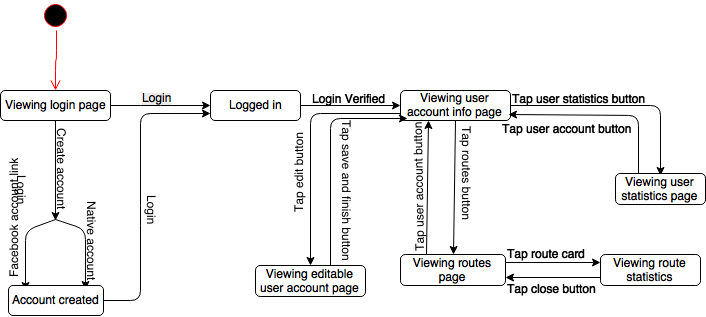
\includegraphics[width=0.8\paperwidth]{creganActivity.png}}
    \end{center}
    \caption{User account system activity diagram}
    \label{fig:my_label}
\end{figure}

\begin{figure}[H]
    \centering
    \begin{center}
        \makebox[\textwidth]{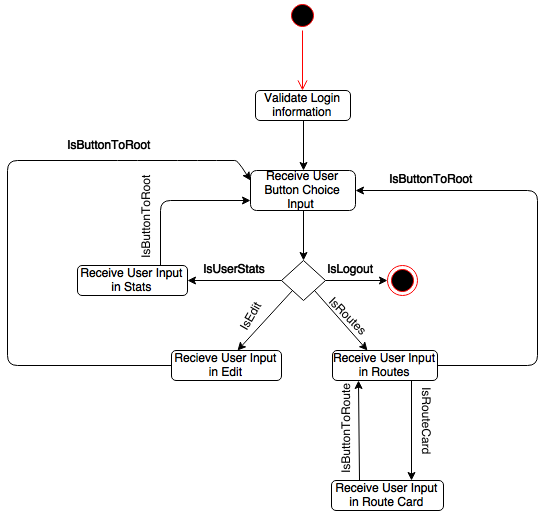
\includegraphics[width=0.8\paperwidth]{creganFlow.png}}
    \end{center}
    \caption{User account dataflow diagram}
    \label{fig:my_label}
\end{figure}

\begin{figure}[H]
    \centering
    \begin{center}
        \makebox[\textwidth]{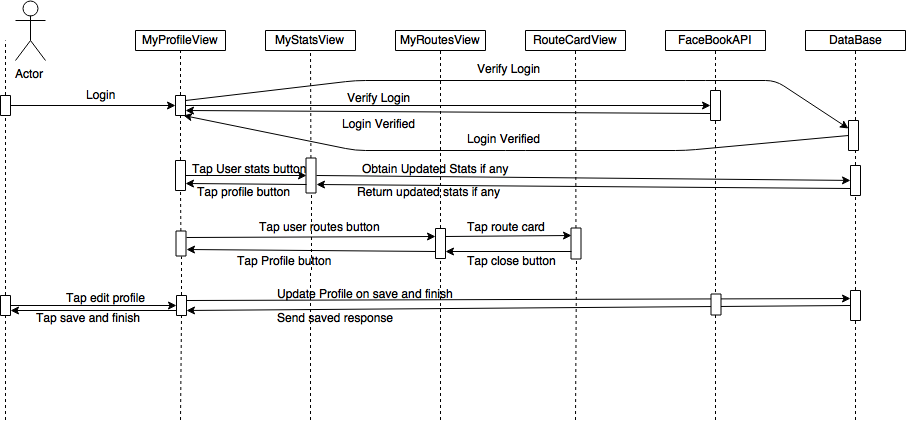
\includegraphics[width=0.8\paperwidth]{creganSeq.png}}
    \end{center}
    \caption{User account sequence diagram}
    \label{fig:my_label}
\end{figure}

\begin{figure}[H]
    \centering
    \begin{center}
        \makebox[\textwidth]{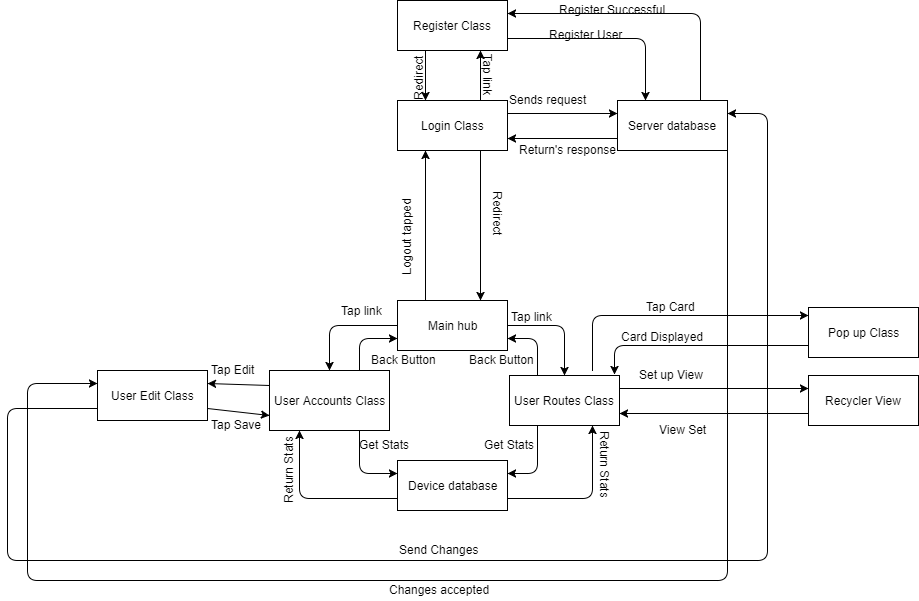
\includegraphics[width=0.8\paperwidth]{creganUML.png}}
    \end{center}
    \caption{User account UML diagram}
    \label{fig:my_label}
\end{figure}

\begin{figure}[H]
    \centering
    \begin{center}
        \makebox[\textwidth]{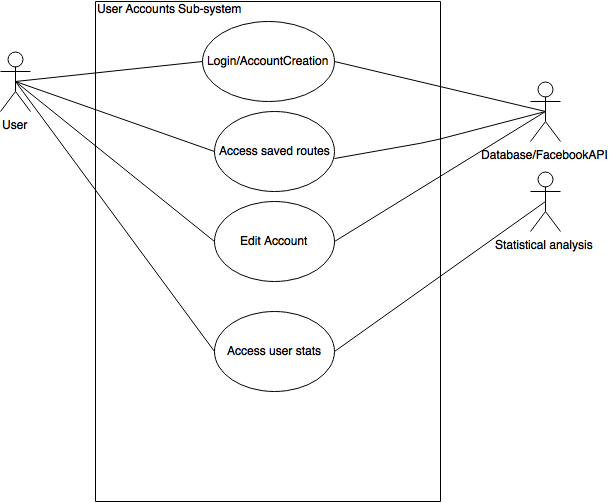
\includegraphics[width=0.8\paperwidth]{creganUseCase.png}}
    \end{center}
    \caption{User account use case diagram}
    \label{fig:my_label}
\end{figure}

\newpage

\subsubsection{Test Cases}
\begin{itemize}
\item TC-01: Login/Create account
\subitem Requirements Fulfilled:
\subsubitem System has implemented UI for login screen and account creation screen and will be connected to singleton authentication method
\subsubitem Singleton authentication system still needs to be linked to database and account creation/login
\subitem Test Steps:
\subsubitem 1. App is started.
\subsubitem 2. Press login after filling valid fields, or press the register link to register then fill the valid fields there and press the register button.
\subsubitem 3. singleton checks the database for user specified by login and returns an accept token to user or if new user registers their info into the database and logs them in with an accept token.
\subitem Expected Result: User is logged in/registered and is added to the database via singleton
\subitem Actual Result: with none of the code linked yet the ui is navigateable and interactable but nothing is added to the database and the user is not actually logged in.
\item TC-02: User account
\subitem Requirements Fulfilled:
\subsubitem User info, stats, and routes page UI all exist.
\subsubitem User info page will display pertinent user account info.
\subsubitem Stats page still in progress on connecting to statistics sub-system and displying information
\subsubitem Routes page has code for route pop up selection will connect to mapping sub-system to allow user to save routes to it as buttons that produce pop ups.
\subitem Test Steps:
\subsubitem 1. App starts.
\subsubitem 2. User logs in/registers.
\subsubitem 3. User is shown account info page.
\subsubitem 4. User selects Stats page and stats are displayed if they have any.
\subsubitem 5. User selects routes page and can tap a saved route veiw a pop up version of it if they have any saved
\subitem Expected Result: the above functionality of the test steps works.
\subitem Actual Result: Stats page does not display stats because not yet linked to stats subsystem, Routes page and pop up work do not display saved routes yet as it is not given a route to display yet, User account page functions as it should.
\end{itemize}

\subsubsection{Login Code so Far}
\begin{lstlisting}[language = Java]
package com.example.daniel.loginregister;

import android.content.Intent;
import android.support.v7.app.AppCompatActivity;
import android.os.Bundle;
import android.view.View;
import android.widget.Button;
import android.widget.EditText;
import android.widget.TextView;

public class LoginActivity extends AppCompatActivity {

    @Override
    protected void onCreate(Bundle savedInstanceState) {
        super.onCreate(savedInstanceState);
        setContentView(R.layout.activity_login);

        final EditText etUsername = (EditText) findViewById(R.id.etUsername);
        final EditText etPassword = (EditText) findViewById(R.id.etPassword);
        final Button bLogin = (Button) findViewById(R.id.bLogin);
        final TextView registerLink = (TextView) findViewById(R.id.tvRegisterHere);

        registerLink.setOnClickListener(new View.OnClickListener() {
            @Override
            public void onClick(View v){
                Intent registerIntent = new Intent(LoginActivity.this, RegisterActivity.class);
                LoginActivity.this.startActivity(registerIntent);
            }
        });
    }
}
\end{lstlisting}

\subsubsection{Registration Code So Far}
\begin{lstlisting}[language = Java]
package com.example.daniel.loginregister;

import android.support.v7.app.AppCompatActivity;
import android.os.Bundle;
import android.widget.Button;
import android.widget.EditText;

public class RegisterActivity extends AppCompatActivity {

    @Override
    protected void onCreate(Bundle savedInstanceState) {
        super.onCreate(savedInstanceState);
        setContentView(R.layout.activity_register);

        final EditText etUsername = (EditText) findViewById(R.id.etUsername);
        final EditText etAge = (EditText) findViewById(R.id.etAge);
        final EditText etEmail = (EditText) findViewById(R.id.etEmail);
        final EditText etWeight = (EditText) findViewById(R.id.etWeight);
        final EditText etSex = (EditText) findViewById(R.id.etSex);
        final EditText etPassword = (EditText) findViewById(R.id.etPassword);
        final Button bRegister = (Button) findViewById(R.id.bRegister);
    }
}
\end{lstlisting}

\subsubsection{User Account Info Page Code So Far}
\begin{lstlisting}[language = Java]
package com.example.daniel.loginregister;

import android.support.v7.app.AppCompatActivity;
import android.os.Bundle;
import android.widget.EditText;

public class UserPage extends AppCompatActivity {

    @Override
    protected void onCreate(Bundle savedInstanceState) {
        super.onCreate(savedInstanceState);
        setContentView(R.layout.activity_user_page);

        final EditText etEmail = (EditText) findViewById(R.id.etEmail);
        final EditText etUsername = (EditText) findViewById(R.id.etUsername);
        final EditText etAge = (EditText) findViewById(R.id.etAge);
        final EditText etSex = (EditText) findViewById(R.id.etSex);
        final EditText etWeight = (EditText) findViewById(R.id.etWeight);
    }
}
\end{lstlisting}

\subsubsection{Routes Page and Button Pop Up Code So Far}
\begin{lstlisting}[language = Java]
package com.pathway.pathway_android;

import android.content.Intent;
import android.support.v7.app.AppCompatActivity;
import android.os.Bundle;
import android.view.View;
import android.widget.Button;

public class routespopup extends AppCompatActivity {

    @Override
    protected void onCreate(Bundle savedInstanceState) {
        super.onCreate(savedInstanceState);
        setContentView(R.layout.activity_routespopup);
        Button route = (Button) findViewById(R.id.route);
        route.setOnClickListener(new View.OnClickListener(){
            @Override
            public void onClick(View v){
                startActivity(new Intent(routespopup.this, routepop.class));
            }
        });
    }
}

package com.pathway.pathway_android;

import android.app.Activity;
import android.os.Bundle;
import android.util.DisplayMetrics;

/**
 * Created by Daniel on 10/20/2017.
 */

public class routepop extends Activity {
    @Override
    protected void onCreate(Bundle savedInstanceState){
        super.onCreate(savedInstanceState);
        setContentView(R.layout.routepopwin);
        DisplayMetrics dm = new DisplayMetrics();
        getWindowManager().getDefaultDisplay().getMetrics(dm);
        int width = dm.widthPixels;
        int height = dm.heightPixels;
        getWindow().setLayout((int)(width*.8), (int)(height*.6));
    }
}
\end{lstlisting}

\subsubsection{Singleton Code So Far}
\begin{lstlisting}[language = Python]
import django


class OnlyOne:

  class __OnlyOne:

    def __init__(self, arg):

      self.val = arg

    def __str__(self):

      return repr(self) + self.val

  instance = None

  def __init__(self, arg):

    if not OnlyOne.instance:

      OnlyOne.instance = OnlyOne.__OnlyOne(arg)

    else:

      OnlyOne.instance.val = arg

  def __getattr__(self, name):

    return getattr(self.instance, name)

  def createuser(username, password):

    user = User.object.create_user(username, password)

    user = authenticate(username, password)

    if user is not None:

      login(request, user)

      #backend authenticates

    #else:


  def userlogin(request, username, password):

    user = authenticate(username, password)

    if user is not None:

      login(request, user)

      #backend authenticates

    #else:


  def passwordchange(username, password):

    user = User.objects.get(username)

    user.set_password(password)

    user.save()

  def logout_view(request):

    logout(request)

    #redirect goes here


\end{lstlisting}

\section{Pathway - Platform}
\begin{itemize}
    \item The system will be developed using Android v5 (Lollipop).
    \item The system will be developed in Android Studio.
    \item The system will employ the Google Maps API in development.
\end{itemize}

\section{Pathway - Domain Analysis}
This document serves as an overview for the planned development of a software system, named Pathway, that is intended to address the difficulties in staying motivated to exercise by incorporating elements of social interaction and friendly competition as a means to motivate through a mobile application interface.

\paragraph{Pathway - Extensions}
\begin{itemize}
    \item Increased social networking functionality.
    \item More detailed performance analytics.
    \item A companion website for profile management, advanced performance display options and tools.
    \item Additional functionality to allow a user to track nutrition intake and plan meals.
    \item Addition of workout tracking and planning such as weight lifting routines.
\end{itemize}

\paragraph{Pathway - General Domain Knowledge}
\begin{itemize}
    \item Users interested in tracking fitness routes have other options, but those applications are often limited in functionality beyond data collection.
    \item Meaningful analysis requires exporting of data or manual input into an outside system.
    \item While many individuals like to share their workout information on social media sites, there does not currently exist an integrated fitness oriented social networking option.
    \item Finding new routes to walk/run/cycle for a user, especially in a new area, can be difficult. Users may solicit advice for where to try these activities on social media.
    \item Users may also elect to try new areas with no prior knowledge.
\end{itemize}

\paragraph{Pathway - Clients and Users}
Target users would include all individuals that:
\begin{itemize}
    \item Are capable of operating a device that is compatible with Pathway.
    \item Are interested in exercising and making connections.
\end{itemize}

\paragraph{Pathway - Computing Environment}
Primary functionality will be developed for Android 5.0 (Lollipop) and as such will be unsupported on version of Android prior to 5.0. Specific system requirements are not yet determined. No additional client requirements will be necessary for database and server access, other than an active network connection.

\subsection{Pathway - Tasks and Procedures}
Currently the general process of selecting a route to traverse (walk, run, or cycle) and then sharing information goes as follows:
\begin{enumerate}
    \item A user solicits route information from friends and acquaintances.
        \begin{itemize}
            \item If successful, the user may use an existing application to log route and speed information.
            \item This information can be exported to an application, such as excel, and analyzed.
            \item A user may elect to also post performance information through social media, such as Facebook.
        \end{itemize}
    \item A user can elect to try a new route.
        \begin{itemize}
            \item A route could be to the user's liking and fitness level, making it more likely that that the route will be completed and traversed again in the future .
            \item If the route is difficult or unpleasant, the user may not finish their planned traversal of the route.
        \end{itemize}
    \item A user may use a $3^rd$ party application to find a group with which to walk or run or bike with.
        \begin{itemize}
            \item This method has the advantage of added support from the group.
            \item The user is more likely to finish and even more likely to perform better than if alone.
        \end{itemize}
\end{enumerate}

\subsection{Pathway - Competing Software}
The following applications/software may fulfill similar roles or offer similar functionality as that proposed in this document for Pathway:
\begin{itemize}
    \item MyTracks - Offers only basic data collection (Lat/Long position, elevation) dependent on device sensors, and no analysis options.
    \item FitBit App - Offers data collection and basic analysis of user performance.
    \item iOS Health - Offers basic data collection and limited analysis of performance.
    \item LG Health - Offers route tracking and calorie journal. Still lacks any social networking component.
\end{itemize}

\subsection{Pathway - Similar Domains}
Many applications are similar to Pathway in the sense that they make use of geospatial data location and/or social networking user accounts. While no other application we found combines all aspects of our project in the same way we do, it will be worthwhile to look at other applications, such as Waze, Facebook, etc to gather some understanding of how to efficiently implement these systems.

\section{Glossary}
\begin{itemize}
    \item \textbf{Route} - A Route in Pathway will be the geometric representation of a user’s tracked traversal path and will include geographic data that defines an exact geographic position through $XY$ coordinates and elevation.
    \item \textbf{Challenge} - A Challenge in Pathway will be the primary means of social interaction between users, acting as a prompt from User A to User B to encourage participation in an exercise activity.
    \item REST API - Representational State Transfer, provides interoperability between systems through the web.
    \item \textbf{Python} - Python is an interpreted, object-oriented programming language similar to PERL.
    \item \textbf{Flask} - Flask is a microframework for Python based on Werkzeug, Jinja 2 and good intentions.
    \item \textbf{MySQL} - MySQL is an open source relational database management system (RDBMS) based on Structured Query Language (SQL).
    \item \textbf{Object Relational Mapping (ORM)} - Object-relational mapping (ORM, O/RM, and O/R mapping tool) in computer science is a programming technique for converting data between incompatible type systems using object-oriented programming languages.
    \item \textbf{Docker} - The Docker Engine is the underlying client-server tool that supports container technology to handle the tasks and workflows involved in building container-based applications.
    \item \textbf{Amazon Web Services (AWS)} - Amazon Web Services (AWS) is a comprehensive, evolving cloud computing platform provided by Amazon.com.
    \item \textbf{scalable} - It is the ability of a computer application or product (hardware or software) to continue to function well when it (or its context) is changed in size or volume in order to meet a user need.
    \item \textbf{dockerize} - The act of containing a piece of software within a docker container.
    \item \textbf{Route} - A Route in Pathway will be the geometric representation of a user’s tracked traversal path and will include data that defines an exact geographic position through XY coordinates and elevation.
    \item \textbf{Challenge} - A Challenge in Pathway will be the primary means of social interaction between users, acting as a prompt from User A to User B to encourage participation in an exercise activity.
    \item \textbf{Statistics} - branch of mathematics dealing with the collection, analysis, interpretation, presentation, and organization of data.
    \item \textbf{Database} - application that contains organized collections of data in tables
    \item \textbf{Geolocation} – A specific pair of x and y coordinates as plotted on a spherical surface, allowing the description of an exact geographic location on that sphere.
    \item \textbf{Latitude} – The angular distance of a location in degrees, minutes, and seconds relative to the earth’s equator. Lat is shorthand.
    \item \textbf{Longitude} – The angular distance of a location in degrees, minutes, and seconds relative to the meridian at Greenwich, England. Long is shorthand.
    \item \textbf{Elevation} – A measurement of height above some arbitrary baseline, usually sea-level, expressed most often in feet or meters. Elev. is shorthand.
    \item \textbf{User} – An individual person who maintains a Pathway account.
    \item \textbf{Route} – A series of two or more data points in sequence that comprise the path taken by a user and showing the user’s traversal across an area.
    \item \textbf{Point} – A recorded location, being comprised of Latitude, Longitude, Elevation, and Time, relative to the first recorded point in the series.
\end{itemize}


\section{Bibliography}
\begin{itemize}
    \item -  Django.readthedocs.io. (2017). Using the Django authentication system — Django 2.1.dev20171017153446 documentation. [online] Available at: http://django.readthedocs.io/en/latest/topics/auth/default.html#how-to-log-a-user-in [Accessed 17 Oct. 2017].
    \item -  Cohen, U. (2017). Write your own Android Authenticator. [online] Blog.udinic.com. Available at: http://blog.udinic.com/2013/04/24/write-your-own-android-authenticator/ [Accessed 17 Oct. 2017].
    \item - Docs.djangoproject.com. (2017). django.contrib.auth | Django documentation | Django. [online] Available at: https://docs.djangoproject.com/en/1.11/ref/contrib/auth/ [Accessed 17 Oct. 2017].
    \item - Python-3-patterns-idioms-test.readthedocs.io. (2017). The Singleton — Python 3 Patterns, Recipes and Idioms. [online] Available at: http://python-3-patterns-idioms-test.readthedocs.io/en/latest/Singleton.html [Accessed 17 Oct. 2017].
    \item - Developer.android.com. (2017). HttpURLConnection | Android Developers. [online] Available at: https://developer.android.com/reference/java/net/HttpURLConnection.html [Accessed 13 Nov. 2017].
\end{itemize}


\bibliographystyle{ieeetr}
\bibliography{PathwayBibliography}



\end{document}
